% chapter 4: three trees

In the previous three chapters we have focused on one of the most well-studied phylogenetic network problems to date, the \mh problem. We were given two rooted phylogenetic trees, $T_1$ and $T_2$, on the same set of taxa~$X$, and the goal was to construct a phylogenetic network that contains an image of each of the input trees, while minimizing the hybridization number~$k$ of the network. 


The holy grail for this problem is to develop algorithms that can cope with many input trees and nonbinary input trees~\cite{davidbook} (and to take different causes of incongruence into account, see e.g. \cite{yu2013parsimonious}).  However, thus far most algorithmic research has focused on the simplest possible case: $|\cT|=2$ and both input trees are binary. As we have seen, the comparative tractability of the problem, both in theory and practice, stems from the essentially one-to-one relationship between solutions to the two-tree problem and the \maaf problem. 


For $|\mathcal{T}| > 2$ the situation becomes more complex, however, even when restricted to binary trees %\footnote{For the rest of the introduction we focus only on the case of binary trees -- see \cite{ipco} and \cite{nonbinary} for an overview of recent nonbinary results. The nonbinary case is a generalization of the binary case and therefore inherits all the negative results, but not the positive results, of the binary problem.} 
and $|\mathcal{T}|=3$. The \maaf abstraction weakens significantly and cannot (obviously) be used to generate optimal solutions to the hybridization number problem.  Without the \maaf abstraction it seems that we have to explicitly confront the challenge of actually constructing the hybridization network itself. This is a theoretically daunting challenge, since the space of DAGs is huge. The good news is that for $|\mathcal{T}|>2$ the problem nevertheless remains FPT in $k$ \cite{vanIerselLinz,towards}. The bad news is that none of these results satisfactorily address the problem of actually constructing the network. The FPT result in \cite{vanIerselLinz} gives a quadratic kernel, but does not describe a (good) algorithm for solving the kernel. The bounded-search FPT result in \cite{towards}, based on \cite{KelkScornavacca2011}, does actually construct the network, but has an astronomical running time. The running time is so large because it brute forces over the space of all possible \emph{generators} i.e. possible ``backbone topologies'' of the network~\cite{elusiveness,KelkScornavacca2011}, a space which is not known to be~$\Oh(c^k)$, and continues with a tower of guesses, which is not~$\Oh(c^k)$, for each such generator. At present, therefore, the only FPT algorithms for the case of three binary trees are either kernelizations, or bounded-search algorithms with an exponential dependency on~$k$ with a non-linear exponent. Several exponential-time algorithms do exist, such as \cite{wu2013algorithm} and the algorithm discussed in \cite{vanIerselLinz}, but using them to solve a kernelized hybridization number instance unfortunately does not help for two reasons. Firstly, the size of the best-known kernel (i.e. the number~$n$ of leaves of a kernelized instance) is quadratic, and not linear in~$k$. Secondly, no previously-known exponential-time algorithm has an~$\Oh(c^n)$ running time. Therefore, the challenge is to determine whether an algorithm with running time $\Oh(c^k \poly(n))$ exists for the case of three binary trees.

  %-----------------------------------------------------------------------------
  \begin{figure}[t]
    \centering
    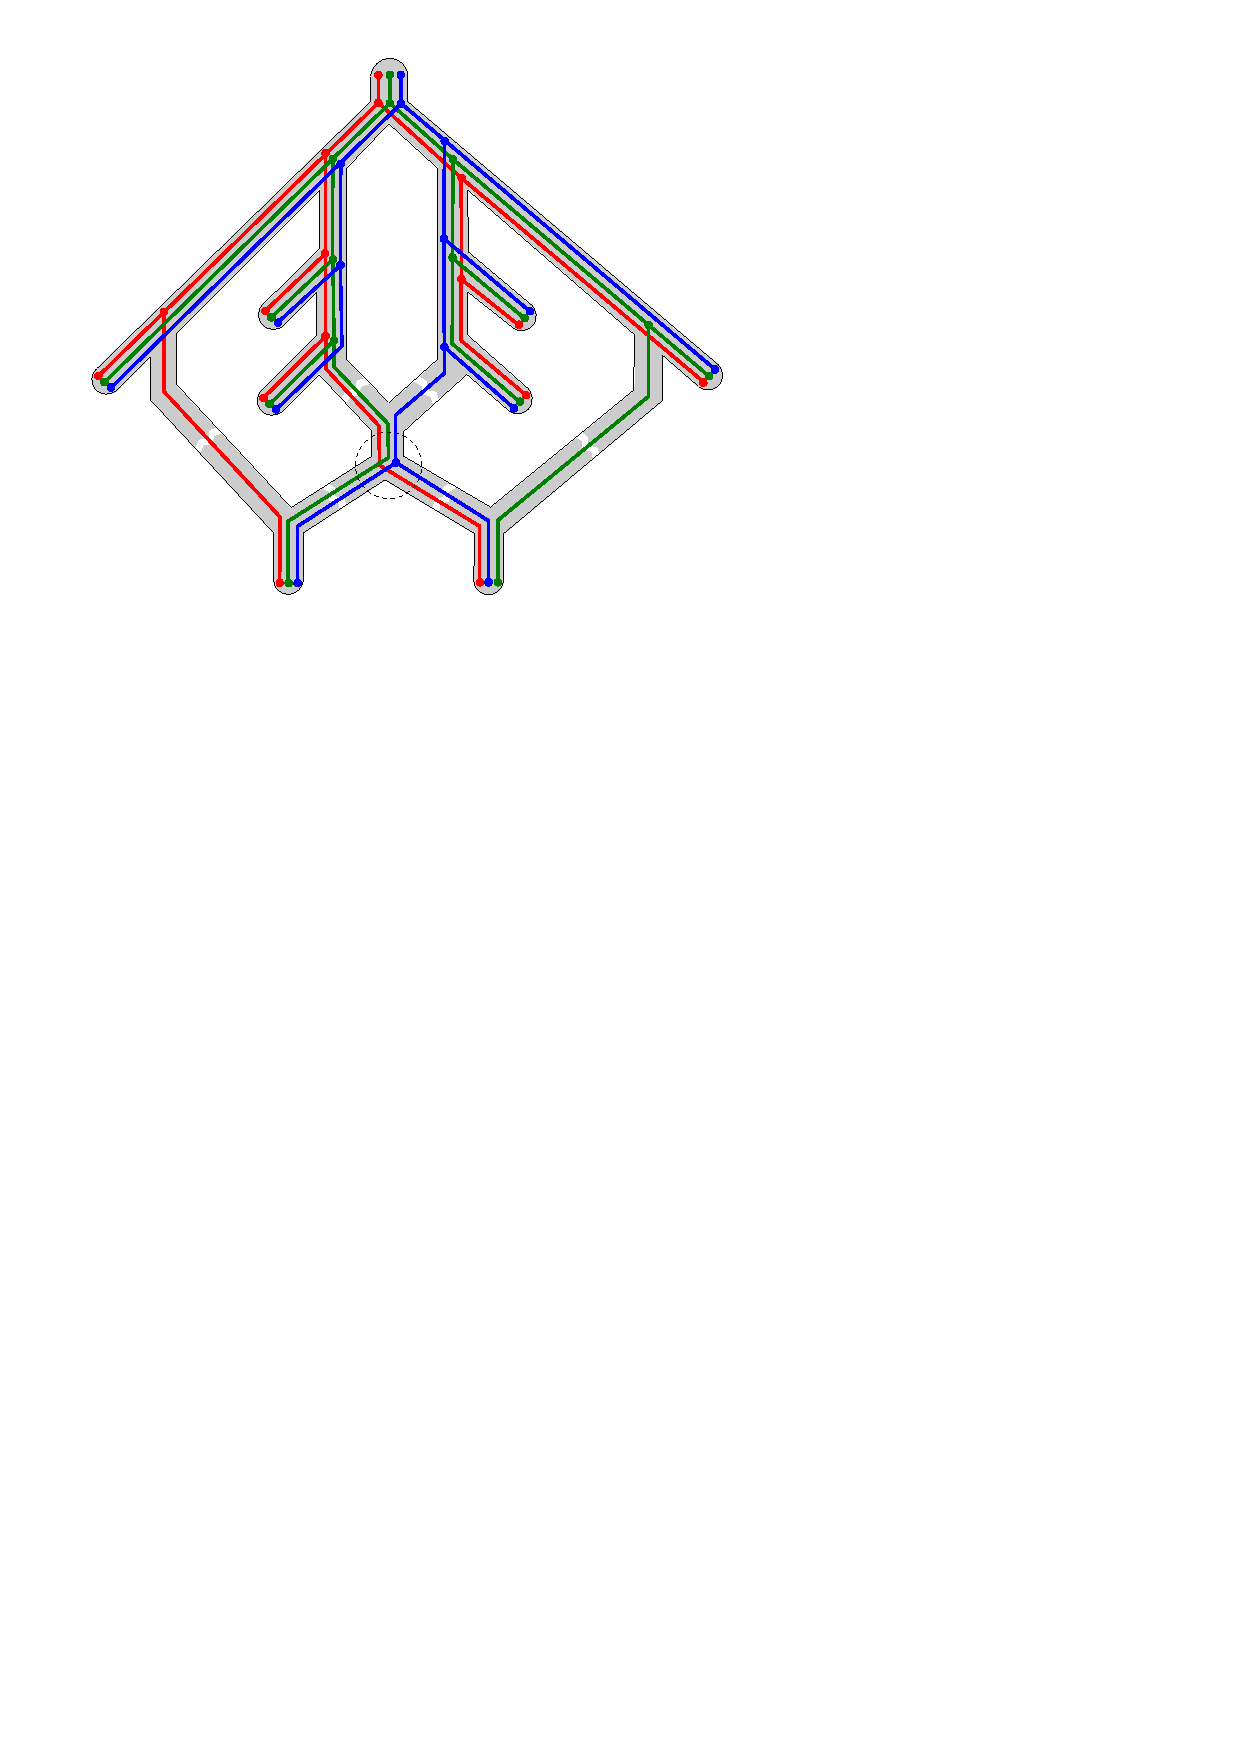
\includegraphics{../figs/ch4/invisible-node-example}
    \caption{A hybridization network for three trees which contains an invisible component (inside the dashed circle), separated from all leaves by hybridization edges (marked with white arrows).   
    It can be shown that any hybridization network for these trees contains an invisible component. However, the single node inside this component can be identified because it corresponds to a node of the blue input tree.}
    \label{fig:invisible}
  \end{figure}
  %-----------------------------------------------------------------------------

In this chapter we answer this challenge positively. Although the constant $c$ that we find is astronomical  - 1609891840 - it represents a significant development in our understanding of the underlying combinatorial structure of the hybridization number problem. We show that, although it is not clear how a \maaf can be pieced together into an optimal solution to the hybridization number problem, it is still possible to identify in $\Oh(c^k \poly(n))$ time a (not necessarily maximum) acyclic agreement forest (AAF) that does have this property. Having found the appropriate acyclic agreement forest, we use deep\comment{LI}{novel?} insights into the structure of optimal hybridization networks to piece the components of the forest together into a network. 

The difficulty of this step comes from the fact that, unlike in the two-tree case, it is no longer possible to avoid having nodes in the network that are separated from all leaves by hybridization edges (which are simply the incoming edges to the reticulation vertices). These nodes are therefore not represented in the agreement forest and this was our motivation for calling them ``invisible'', see Figure~\ref{fig:invisible}. The main insight helping to overcome this problem is that, in the case $|\mathcal{T}|=3$, there always exists an optimal hybridization network such that each of its outdegree-2 nodes corresponds to one or more outdegree-2 nodes of the input trees. This enables us to keep the combinatorial explosion in the number of possible network topologies under control. 


Note that our algorithm can be viewed as a structural generalisation of existing algorithms for two trees, which also separate the identification of the underlying acyclic agreement forest and the construction of the network into two phases. In the case of two trees the second phase is polynomial and it is comparatively easy to obtain $\Oh(c^k \poly(n))$  running times for the first phase. In fact, although our overall result at present only  holds for the case $|\mathcal{T}|=3$, the results for the first phase go through without modification for the case $|\mathcal{T}| > 3$. As we demonstrate, the only barrier to extending our result is the fact that, for $|\mathcal{T}|>3$, the combinatorial insight mentioned in the previous paragraph no longer holds. Indeed, there are two new challenges stemming from this result. Firstly, to adapt and generalize the combinatorial insight so that the wider result can be extended to four or more trees. Secondly, to significantly optimize the constant $c$ in our running time. How close can we get to the competitive $\Oh(3.18^k \poly(n))$ running time achieved in the two-tree case?

The structure of the chapter is as follows. We start by ``guessing'' the underlying acyclic agreement forest of an optimal hybridization network in $\Oh(c^k \poly(n))$  time in section~\ref{sec:aaf-guessing}. We then define a notion of canonical networks in Section~\ref{sec:network-to-canonical-network} %(basically, networks of which each outdegree-2 node corresponds to an outdegree-2 node of at least one of the input trees) 
and show that we may restrict to them as long as there are at most three trees in the input. Subsequently, Section~\ref{sec:guessing-things} shows how such a canonical network can be reconstructed from an acyclic agreement forest and the input trees in $\Oh(c^k \poly(n))$ time. Finally, we give an example of the algorithm in Section \ref{sec:example} and present our conclusions in Section~\ref{sec:concl}.





%-------------------------------------------------------------------------------
\section{Guessing the \aaf}\label{sec:aaf-guessing}
%-------------------------------------------------------------------------------

\noindent
{Let~$\T$ be a collection of input trees.} Without loss of generality we will assume that {$\T$ contains} no nontrivial common pendant subtrees. {In this section, we show how we can guess an AAF from which we can build an optimal hybridization network for~$\T$. To make this precise, we define the \emph{deletion forest} of a network~$N$ as} the forest obtained by deleting all the reticulation edges of~$N$, deleting all resulting connected components that do not contain any taxa, and then taking the partition of the taxa induced by the remaining connected components. By this definition a forest is not a set of trees but a partition of taxa set. However, as we did before, we use these two definitions interchangeably as sometimes it is more useful to see a forest as a collection of trees and sometimes as a collection of taxa sets. Note that for a given network the deletion forest is uniquely defined. {We start by proving the following lemma.}

\begin{lem}
  \label{lem:network-to-aaf}
Given a hybridization network~$N$ with hybridization number~$k$ {for a set~$\T$ of input trees}, the deletion forest of~$N$ {is} an AAF of~$\T$ with at most $k+1$ components.
\end{lem}
\begin{proof}
We first show that the deletion forest contains at most $k+1$ components. To see this, note that~$N$ contains exactly~$k$ reticulation nodes. For a reticulation node~$r$, let $X(r)$ be the set of taxa that can be reached from~$r$ by directed paths that start at~$r$ and which do not intersect with any reticulation {apart from~$r$}. (Possibly, $X(r)=\emptyset$.) By construction, none of the edges on these directed paths are deleted when the deletion forest is created. Hence, all the taxa in $X(r)$ will be in the same connected component. Similarly,~{if $X(\rho)$ denotes the set of taxa reachable by directed paths that start at the root and which do not intersect with any reticulations, then the taxa in~$X(\rho)$ will also be together in the same connected component. Note that the deletion forest~$\F$ of~$N$ (seeing it as a partition of the taxa) is the collection containing~$X(\rho)$ if~$X(\rho)\neq\emptyset$ and~$X(r)$ for each reticulation~$r$ for which~$X(r)\neq\emptyset$. Hence, the deletion forest containst at most~$k+1$ components. Moreover, for each~$F\in\F$, each input tree must yield the same subtree when restricted to the subset of taxa of~$F$ because~$N$ displays all the input trees. In addition, for each input tree~$T\in\T$, the subtrees $\{T(L(F)) \mid F\in\F\}$ are node-disjoint, again because~$N$ displays~$T$. It follows that the deletion forest~$\F$ of~$N$ is indeed an AAF of the input trees,
with at most $k+1$ components.}
\end{proof}

As a consequence of Lemma~\ref{lem:network-to-aaf}, we will from now on refer to the deletion forest of a network as its \emph{deletion AAF}. {We can now show how one can guess the deletion AAF of some optimal hybridization network for the input trees.}
%-------------------------------------------------------------------------------
%-------------------------------------------------------------------------------
\begin{lem}
  \label{lem:aaf-to-network}
Let~$k$ be the hybridization number of the {set~$\T$} of input trees. Then, in time
$\Oh(c^k \poly(n))$, we can guess an AAF {that is the deletion AAF of some hybridization network for~$\T$ with hybridization number~$k$}.
\end{lem}
\begin{proof}
{Consider an arbitrary input tree~$T\in\T$. Observe that an AAF of~$\T$ with $k'+1$ components can be obtained from~$T$ by deleting exactly~$k'$ edges and taking the partition of the taxa induced by the resulting connected components. By Lemma~\ref{lem:network-to-aaf}, the deletion AAF of an optimal hybridization network for~$\T$ has at most~$k+1$ components. The goal therefore is to locate the at most~$k$ edges that need to be deleted from~$T$ in order to obtain the deletion AAF of some optimal hybridization network for~$\T$.}

{Let~$N$ be a hybridization network for~$\T$ with hybridization number~$k$ and consider its underlying generator, which is a $k$-reticulation generator and hence has at most~$k$ node sides and at most~$4k-1$ edge sides~\cite{vanIerselLinz}. (For a reminder of these definitions see page~\pageref{sec:kernel}.) It follows that there are at most $5k-1$ common chains of~$\T$, because any two taxa on the same edge side of~$N$ are in the same common chain, as argued in ~\cite{vanIerselLinz}. The} set of common chains is unambiguously defined by the set of input trees, can be computed in polynomial time, and no two chains can share a taxon. {Moreover,} in~\cite{vanIerselLinz} it is proven that if two or more taxa of a common chain are on a single edge side of the underlying generator, the entire chain can safely be moved onto that edge side. That is, the new network still displays the input trees and has hybridization number no higher than the old network.

This means that we can assume the existence of an optimal network $N'$ such that for each common chain there are exactly two possibilities: (1) the chain is on a single {edge side} of the underlying generator, or (2) each taxon of the chain is on a different side of the underlying generator. For each chain we can guess which of the two cases holds, using at most $2^{5k-1}$ guesses for the entire set of chains. {Since, as mentioned before, any two taxa that are on the same side are together in a common chain, it follows that each side of (the underlying generator of)~$N'$ contains either a complete case (1) chain or a single taxon (which is either in a case (2) chain or a singleton-chain) or no taxa at all.}

Now, assume that we have identified the correct set of guesses describing the behaviour of the common chains in~$N'$. It remains to show that we can identify the correct set of edges to delete in~$T$ to obtain the deletion AAF corresponding to $N'$. Observe that for each case (1) chain it is not necessary to delete any of the internal edges of the chain in~$T$. This is because we have correctly identified that the entire chain sits on a single edge side of the generator and thus that it sits inside a single component of the deletion AAF. For all other edges in~$T$ we can simply guess whether to delete it or not. Fortunately, there are not too many of these edges. Specifically, recall that each side contains either a case (1) chain or a single taxon, and that the number of sides is at most $5k-1$. Hence, if we collapse each case (1) chain~$C$ into a new taxon $x_{C}$, which is permitted because we will never cut its internal edges, there are in total at most $5k - 1$ taxa left. A binary tree with $5k-1$ taxa has $10k - 4$ edges. By brute forcing on these edges (i.e. guessing whether to delete it or not) we observe that, in total, the deletion AAF of~$N'$ can be located in time at most $\Oh(2^{5k} \cdot 2^{10k} \cdot \poly(n))$.
\end{proof}

Notice that the proof of Lemma \ref{lem:aaf-to-network} tells us how to find a correct AAF, but it doesn't tell us how to construct an optimal hybridization network from this AAF.
% -*- TeX-master: "main" -*-

%-------------------------------------------------------------------------------
\section{Canonical networks}
%-------------------------------------------------------------------------------

\label{sec:network-to-canonical-network}

In this section we give the only lemma that is three-tree specific. We describe a transformation from a hybridization network to a structure, called a canonical network with embedded trees, that has some desirable properties. We prove that the transformation preserves the hybridization number in the three-tree case, and hence in the three-tree case we are allowed to concentrate on canonical networks only. {For ease of notation, we will sometimes identify a directed graph with its edge set.}

A \emph{Canonical Network with Embedded Trees (CNET)} for a set $\T$ of phylogenetic trees over a label set $X$ is a pair $\H = (H, \E)$ with the following properties:
\begin{enumerate}%[label=(\roman{*}),leftmargin=*,widest=viii,noitemsep]
\item $H$ is a DAG. We call its sources, i.e. indegree-0 nodes, \emph{roots} and its sinks, i.e. outdegree-0 nodes, \emph{leaves}.\label{cond:acyclic-network}
\item Every root of $H$ has one child.\label{cond:non-splitting-roots}
\item The leaves of $H$ are labelled bijectively with the leaf labels in 
  $X$.\label{cond:leaf-labelling}
\item $\E = \set{H(T) \subseteq H \mid T \in \T}$ such that for all $T \in \T$,
  $H(T)$ is an \emph{image} of $T$, that is, $T$ can be obtained from $H(T)$
  by suppressing degree-$2$ nodes.\label{cond:displays-trees}
\item Every tree image $H(T) \in \E$ contains an edge incident to a root of
  $H$.\label{cond:start-at-the-root}
\item $H = \bigcup_{T \in \T}H(T)$, that is, every edge of $H$ belongs to at
  least one tree image in $\E$.\label{cond:no-useless-edges}
\item Every {non-leaf} non-root node of $H$ has exactly two
  children.\label{cond:bifurcating-nodes}
\item For every {non-leaf} non-root node, there exists a tree image
  $H(T) \in \E$ that contains both its child
  edges.\label{cond:every-node-splits}
\end{enumerate}

We represent the tree images in $\E$ by associating a unique colour with each tree $T \in \T$ and colouring every edge in $H(T)$ with this colour. We call the colour associated with tree $T$ \emph{colour $T$}. We use $C(e)$ to denote the colour set of an edge $e$ of $H$, that is, the set of trees $T \in \T$ whose images $H(T) \in \E$ include $e$. A CNET for the input trees in Figure~\ref{fig:reconstruction-input} on page~\pageref{fig:reconstruction-input} is shown in Figure~\ref{fig:reconstruction-output} on page~\pageref{fig:reconstruction-output}. A corresponding hybridization network is shown in Figure~\ref{fig:reconstruction-final} on page~\pageref{fig:reconstruction-final}.

The hybridization network \emph{induced} by a CNET~$(H', \E)$ is the hybridization network obtained by applying the following transformations to $H'$:
  \begin{itemize}%[noitemsep]
  \item We replace every node $x$ that is both a reticulation node and a split
    node with two nodes $x_t$ and~$x_b$, change the bottom endpoints of $x$'s
    parent edges to $x_t$, change the top endpoints of $x$'s child edges to
    $x_b$, and add an edge from $x_t$ to $x_b$.
  \item We replace every reticulation node with more than two parents with a
    chain of binary reticulation nodes. {See Figure~\ref{fig:nodesplit} for an illustration of these first two steps.}
  \item As long as there are at least two roots, we choose two such roots $r_1$
    and $r_2$, change the top endpoint of $r_1$'s child edge to $r_2$, and add
    an edge from $r_1$ to $r_2$. 
		This reduces the number of roots by one, so we eventually obtain a network
    with a single root. See Figure \ref{fig:rootjoin}.
\item For every leaf $x$ with more than one parent, we create a new
    node $x'$, change the bottom endpoint of every parent edge of $x$ to $x'$,
    and add an edge from $x'$ to $x$.
  \end{itemize}
	
\begin{figure}[h]
	\centering
		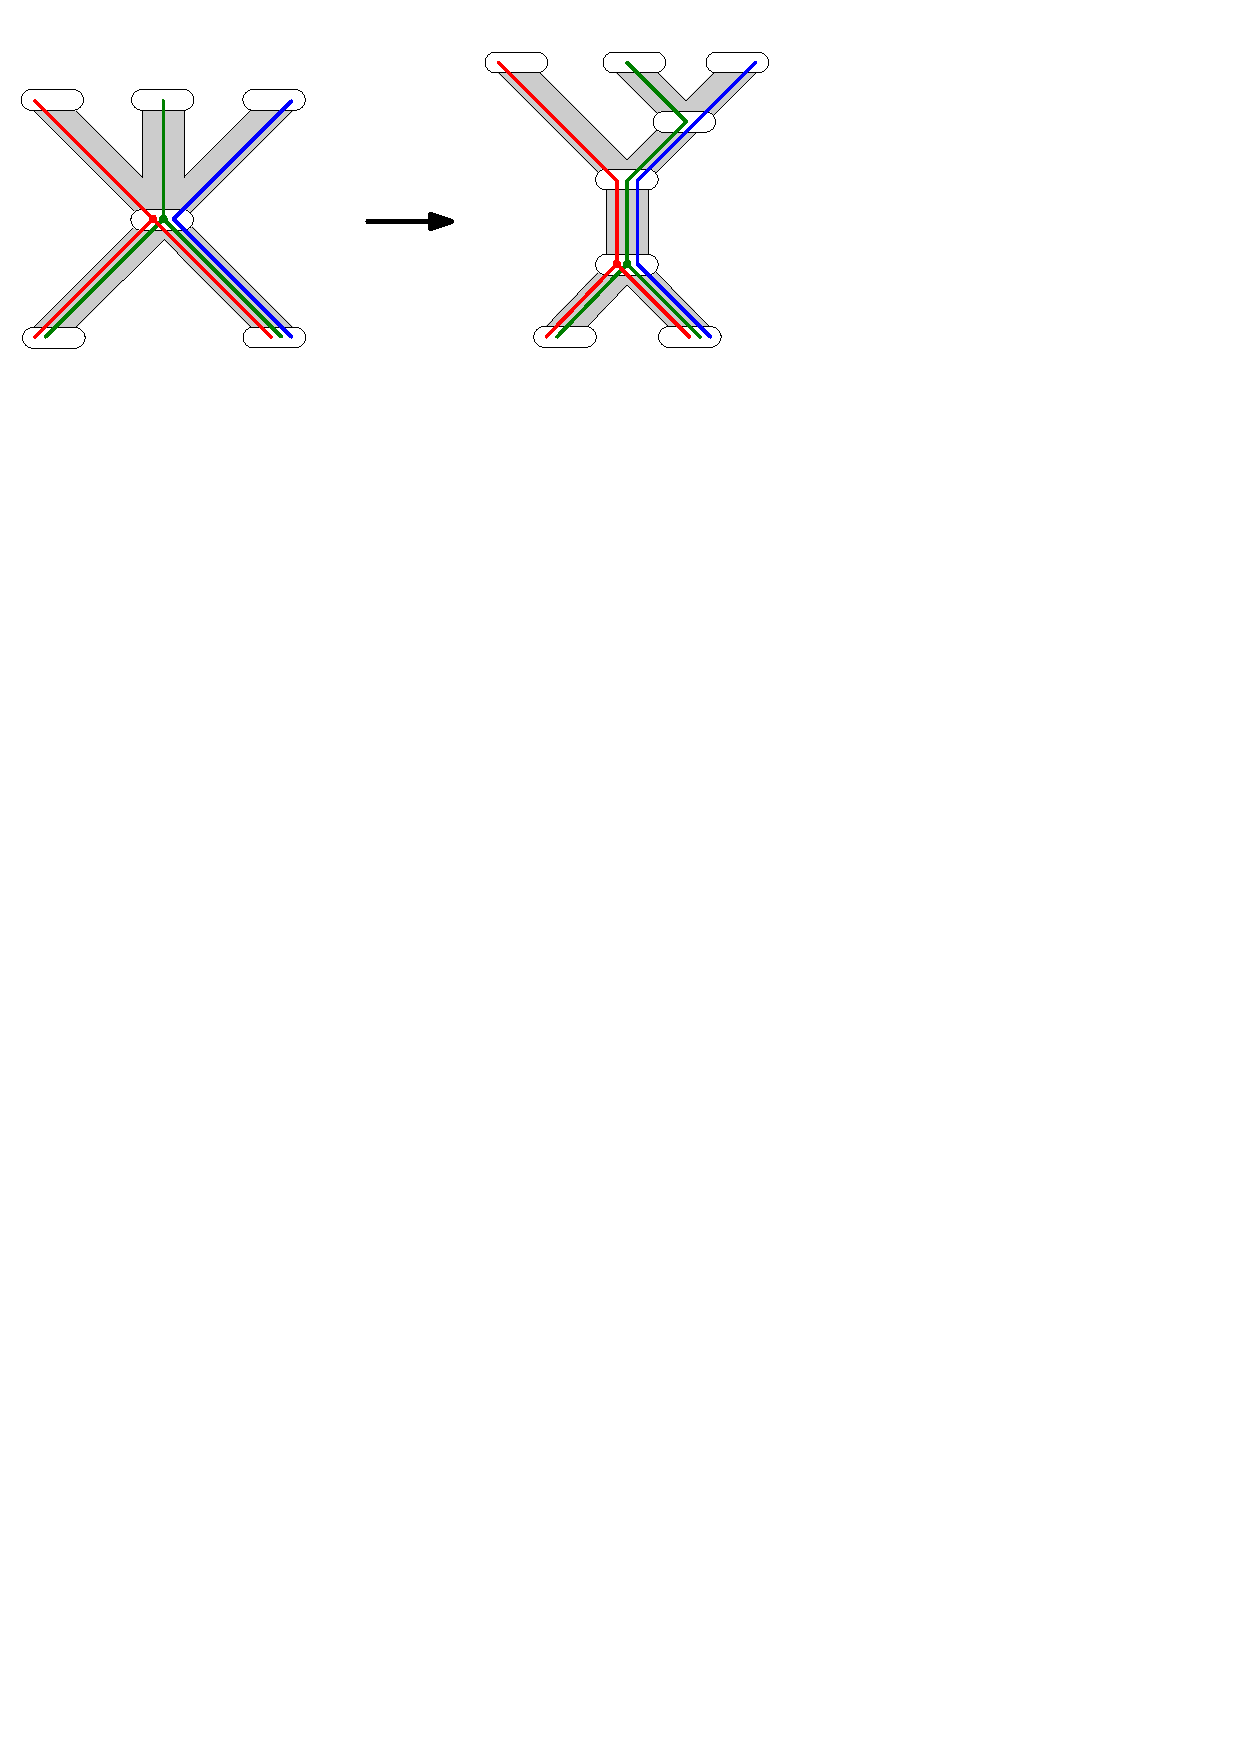
\includegraphics{../figs/ch4/node-splitting2.pdf}
	\caption{The first two steps of transforming a CNET into a hybridization network: expanding nodes that are both reticulation and split nodes and refining reticulations.}
	\label{fig:nodesplit}
\end{figure}

\begin{figure}[h]
	\centering
		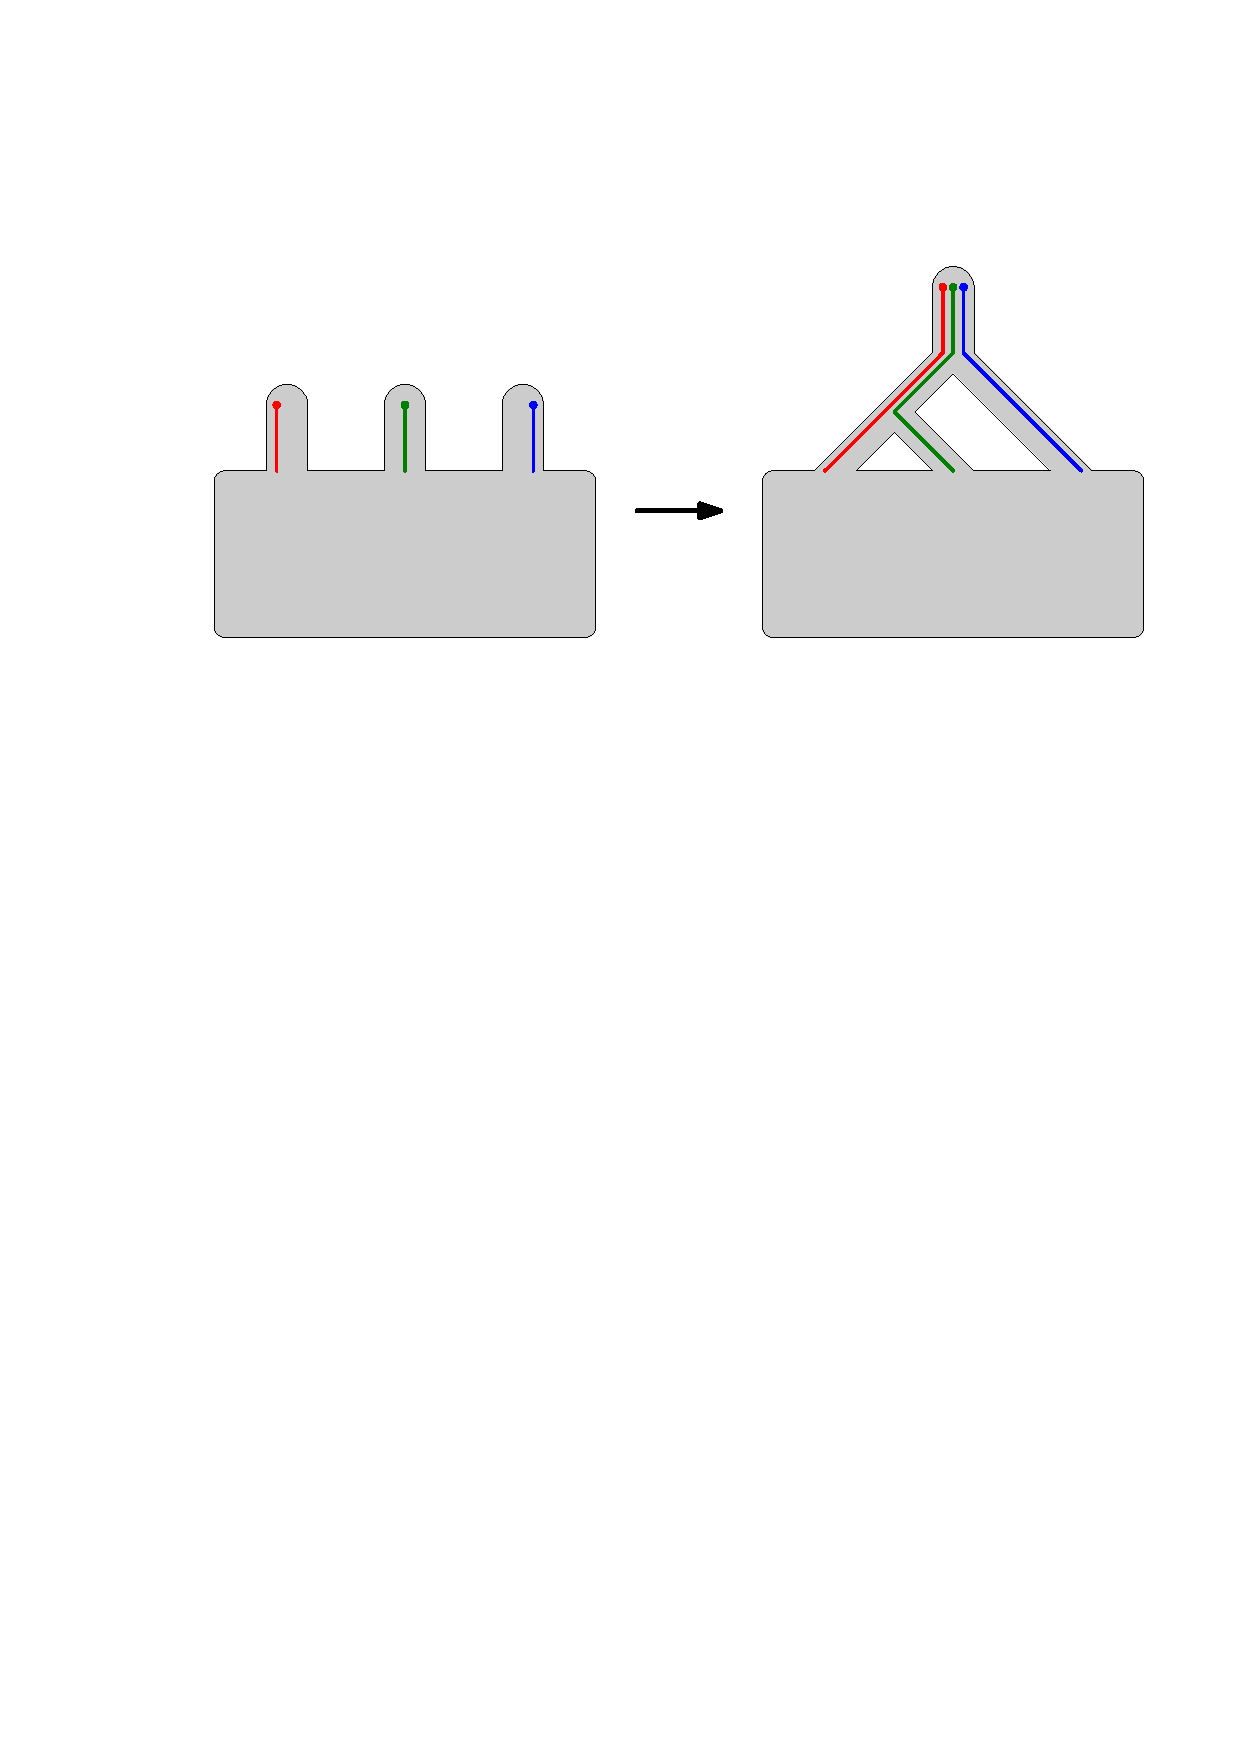
\includegraphics{../figs/ch4/root-joining.pdf}
	\caption{The third step of transforming a CNET into a hybridization network: combining multiple roots.}
	\label{fig:rootjoin}
\end{figure}

The \emph{deletion AAF} of a CNET~$(H, \E)$ is defined to be the deletion AAF of the hybridization network induced by~$(H, \E)$. {The \emph{hybridization number} of a CNET~$(H, \E)$ is (as for networks) defined to be the sum $\sum(d^-(v)-1)$ over all nodes~$v$ of~$H$ with indegree $d^-(v)$ at least~1 i.e. over all non-roots.}

%-------------------------------------------------------------------------------
\begin{lem}
  \label{lem:multiroot-is-fine}
  If $\size{\T} = 3$, then there exists a hybridization network~$H$ with
  hybridization number $k$ for $\T$ if and only if there exists a
  CNET $\H = (H', \E)$ with hybridization number $k$ for $\T$. Moreover, if such~$H$ and~$\H$ exist then they have the same deletion AAF.
\end{lem}
%-------------------------------------------------------------------------------

\begin{proof}
  First suppose that there exists a CNET $\H = (H', \E)$ with hybridization number $k$ for $\T$. Then, the hybridization network~$H$ induced by~$\H$ has the same hybridization number as $H'$, and it is easy to see that $H$ displays the trees in $\T$,   given that $H'$ displays these trees. It follows directly from the definition of the deletion AAF of a CNET that~$H$ and~$\H$ have the same deletion AAF.

  Now assume we are given a hybridization network $H$ with hybridization number $k$ for $\T$. Since $H$ displays all trees in $\T$, we can choose a tree image $H(T)$, for every tree $T \in \T$, that includes the root of~$H$. Then we set $\H = (H, \E)$. $\H$ satisfies conditions~\ref{cond:acyclic-network}--\ref{cond:start-at-the-root} of a CNET but may violate the remaining three conditions. Next we describe transformations that we apply to $\H$ to ensure it satisfies these remaining conditions without introducing any violations of the conditions $\H$ already satisfies and without increasing the hybridization number of $\H$. Thus, after applying these transformations, we obtain a {CNET} with hybridization number at most $k$ for~$\T$.

  %-----------------------------------------------------------------------------
  \paragraph{Condition~\ref{cond:no-useless-edges}.}
  %-----------------------------------------------------------------------------

  Deleting all edges of $H$ that are not contained in $\bigcup_{T \in \T}H(T)$   does not violate   conditions~\ref{cond:acyclic-network}--\ref{cond:start-at-the-root}\comment{LI}{Note that this cannot create new leaves because then the edge entering the new leaf would also have been deleted.} and   establishes condition~\ref{cond:no-useless-edges}.   Since it also does not increase the hybridization number of~$\H$, we obtain   a network with hybridization number at most $k$  that satisfies conditions 
  \ref{cond:acyclic-network}--\ref{cond:no-useless-edges}.

  %-----------------------------------------------------------------------------
  \paragraph{Condition~\ref{cond:bifurcating-nodes}.}
  %-----------------------------------------------------------------------------

  As long as there is a \emph{non-splitting} non-root node $x$, that is, a   non-root node with only one child, we contract the edge $e$ between $x$ and   its child in $H$ and in every tree image $H(T) \in \E$ that includes $e$, and   merge any parallel edges this may create. Each such contraction reduces the number of non-splitting non-root nodes by   one, does not introduce any violations of   conditions~\ref{cond:acyclic-network}--\ref{cond:no-useless-edges}, and does   not increase the hybridization number of~$\H$.   Thus, we eventually obtain a network with hybridization number at most $k$   that satisfies   conditions~\ref{cond:acyclic-network}--\ref{cond:bifurcating-nodes}.

  %-----------------------------------------------------------------------------
  \paragraph{Condition~\ref{cond:every-node-splits}.}
  %-----------------------------------------------------------------------------

  By condition~\ref{cond:bifurcating-nodes}, every non-root node of $H$ is a   split node.   We call it a \emph{true split node} if it also satisfies   condition~\ref{cond:every-node-splits}, and a \emph{fake split node}   otherwise.   We also call a true split node {a \emph{$T$-split node} if the tree image~$H(T)$ contains both its child edges.}   The \emph{weight} of a node $x$ is the number of trees $T \in \T$ such that   $x$ is a $T$-split node. The \emph{weight} of a path is the sum of the weights of the nodes on the path. Now we define the \emph{potential} $\phi_x$ of a fake split node to be one plus the maximum weight of a path from a root to $x$. {All} other nodes have potential $0$.   The potential of the network is $\Phi := \sum_x \phi_x$, where the sum is   taken over all nodes of the network.   Since every fake split node has a positive potential, a network has potential $\Phi = 0$ if and only if it contains no fake split node, that is, if and only if it satisfies condition~\ref{cond:every-node-splits}.   Next we describe a transformation that decreases the potential of the network   without increasing its hybridization number or introducing any violations   of conditions~\ref{cond:acyclic-network}--\ref{cond:bifurcating-nodes}.   Thus, {after repeating this transformation as often as possible, we} obtain a network with   hybridization number at most $k$ which satisfies  conditions~\ref{cond:acyclic-network}--\ref{cond:every-node-splits}, so it  is a CNET with hybridization number at most $k$   for~$\T$.

  While the network contains fake split nodes, there exists such a node $x$ all of whose ancestors are true split nodes or roots.   (Simply remove all roots, true split nodes, and leaves from $H$ and choose   $x$ to be an in-degree-$0$ node of the resulting subgraph of $H$.)   Since the colour sets of $x$'s child edges are disjoint and $x$ has two child   edges, one of these edges, $e$, must have exactly one colour:   $C(e) = \set{T}$, for some $T \in \T$.\footnote{This is the only place where we use that $\size{\T} = 3$.  All other arguments are easily seen to generalize to more than $3$ trees.     Alas, this argument is crucial because our algorithm does not work without     condition~\ref{cond:every-node-splits}.}   Let $f$ be $x$'s parent edge that has colour $T$.   By the choice of $x$, the top endpoint $y$ of $f$ is a root or a true split   node.

  %-----------------------------------------------------------------------------
  \begin{figure}
    \centering
    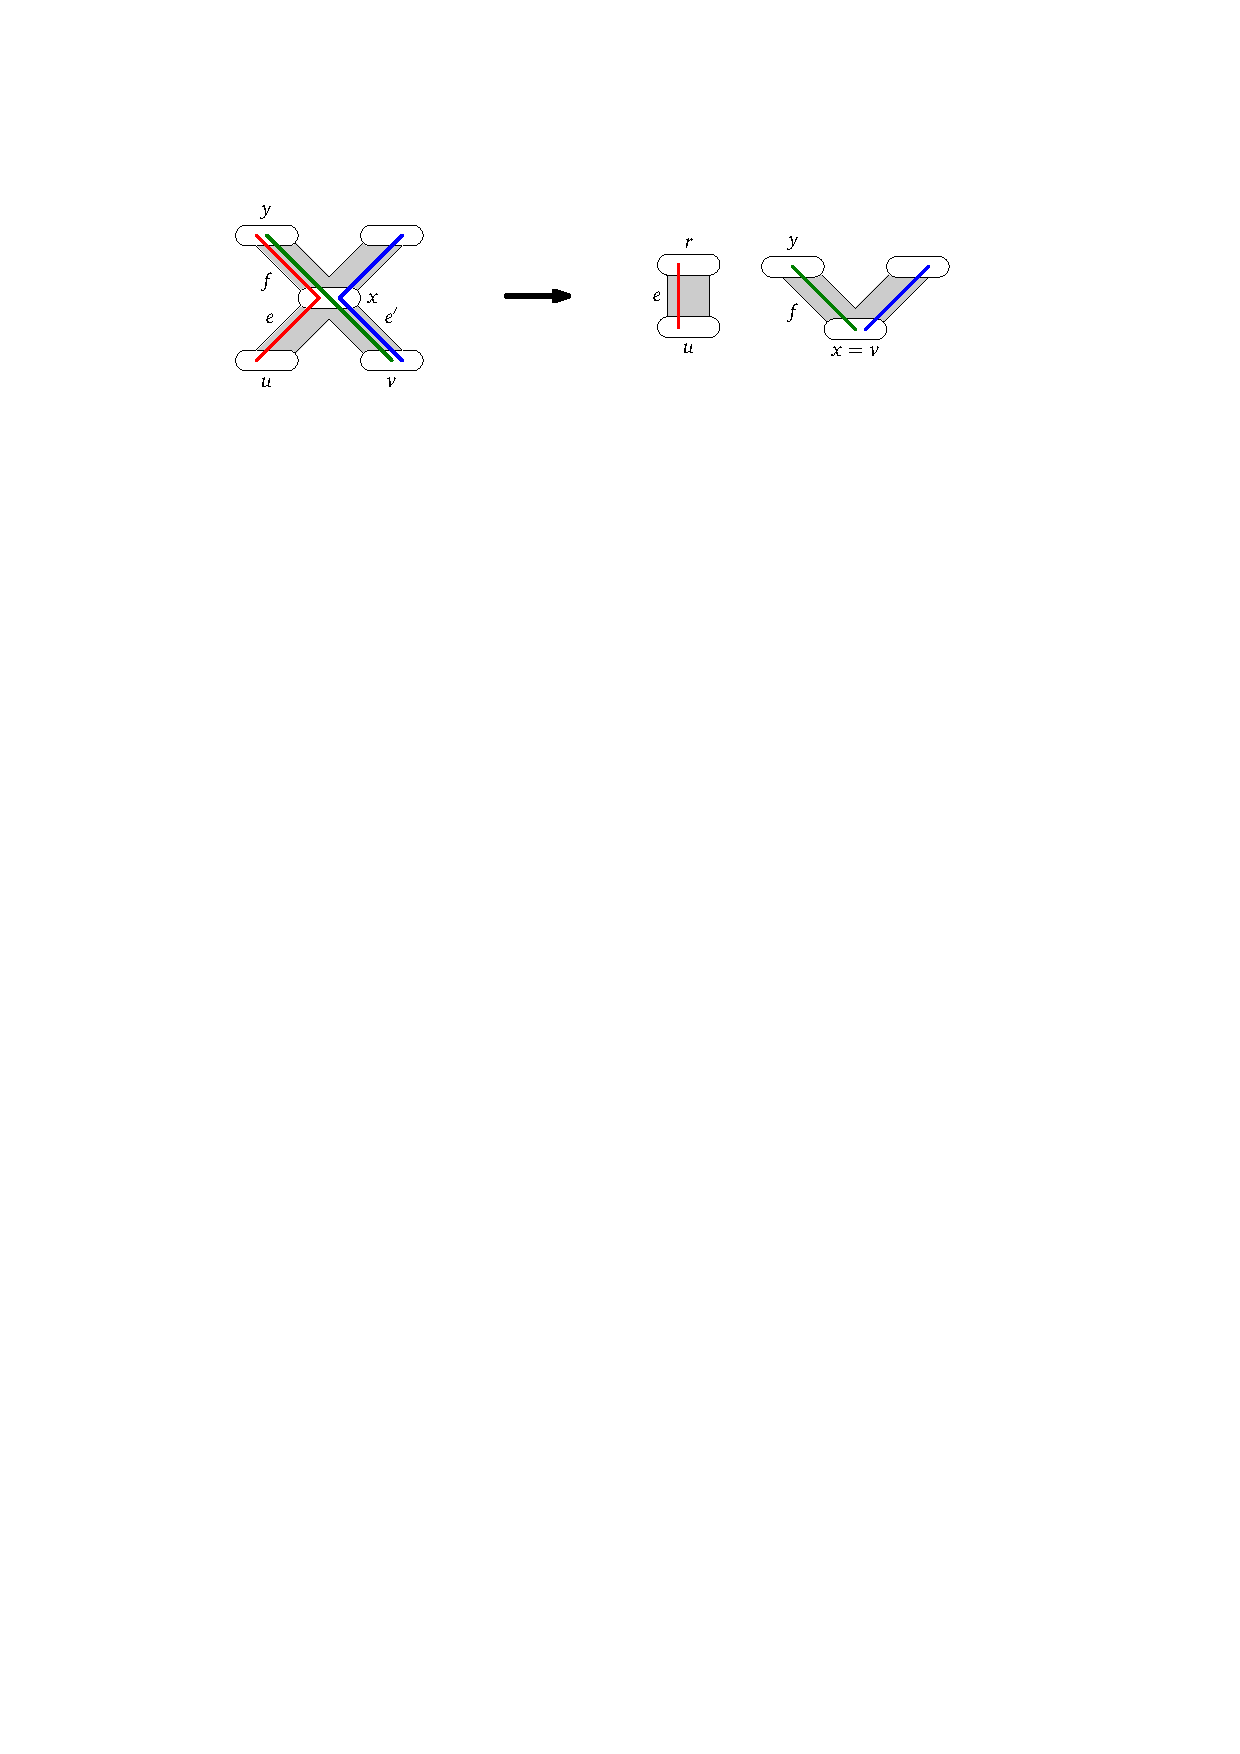
\includegraphics{../figs/ch4/root-transformation}
    \caption{Eliminating a fake split node $x$ below a root $y$.}
    \label{fig:root-transformation}
  \end{figure}
  %-----------------------------------------------------------------------------

  If $y$ is a root (see Figure~\ref{fig:root-transformation}), we remove $T$   from the colour set of $f$, create a new root   node $r$, change $e$'s top endpoint to $r$, remove $f$ and its top   endpoint{~$y$ if the colour set of~$f$} is now empty and restore Condition~\ref{cond:bifurcating-nodes}.   It is easily verified that this does not introduce any violations of   conditions~\ref{cond:acyclic-network}--\ref{cond:no-useless-edges} and   does not increase the hybridization number of the network.   {It also does not increase the potential of any node, and reduces the number of fake split nodes by one. The} potential of the network therefore decreases.

  %-----------------------------------------------------------------------------
  \begin{figure}
    \centering
    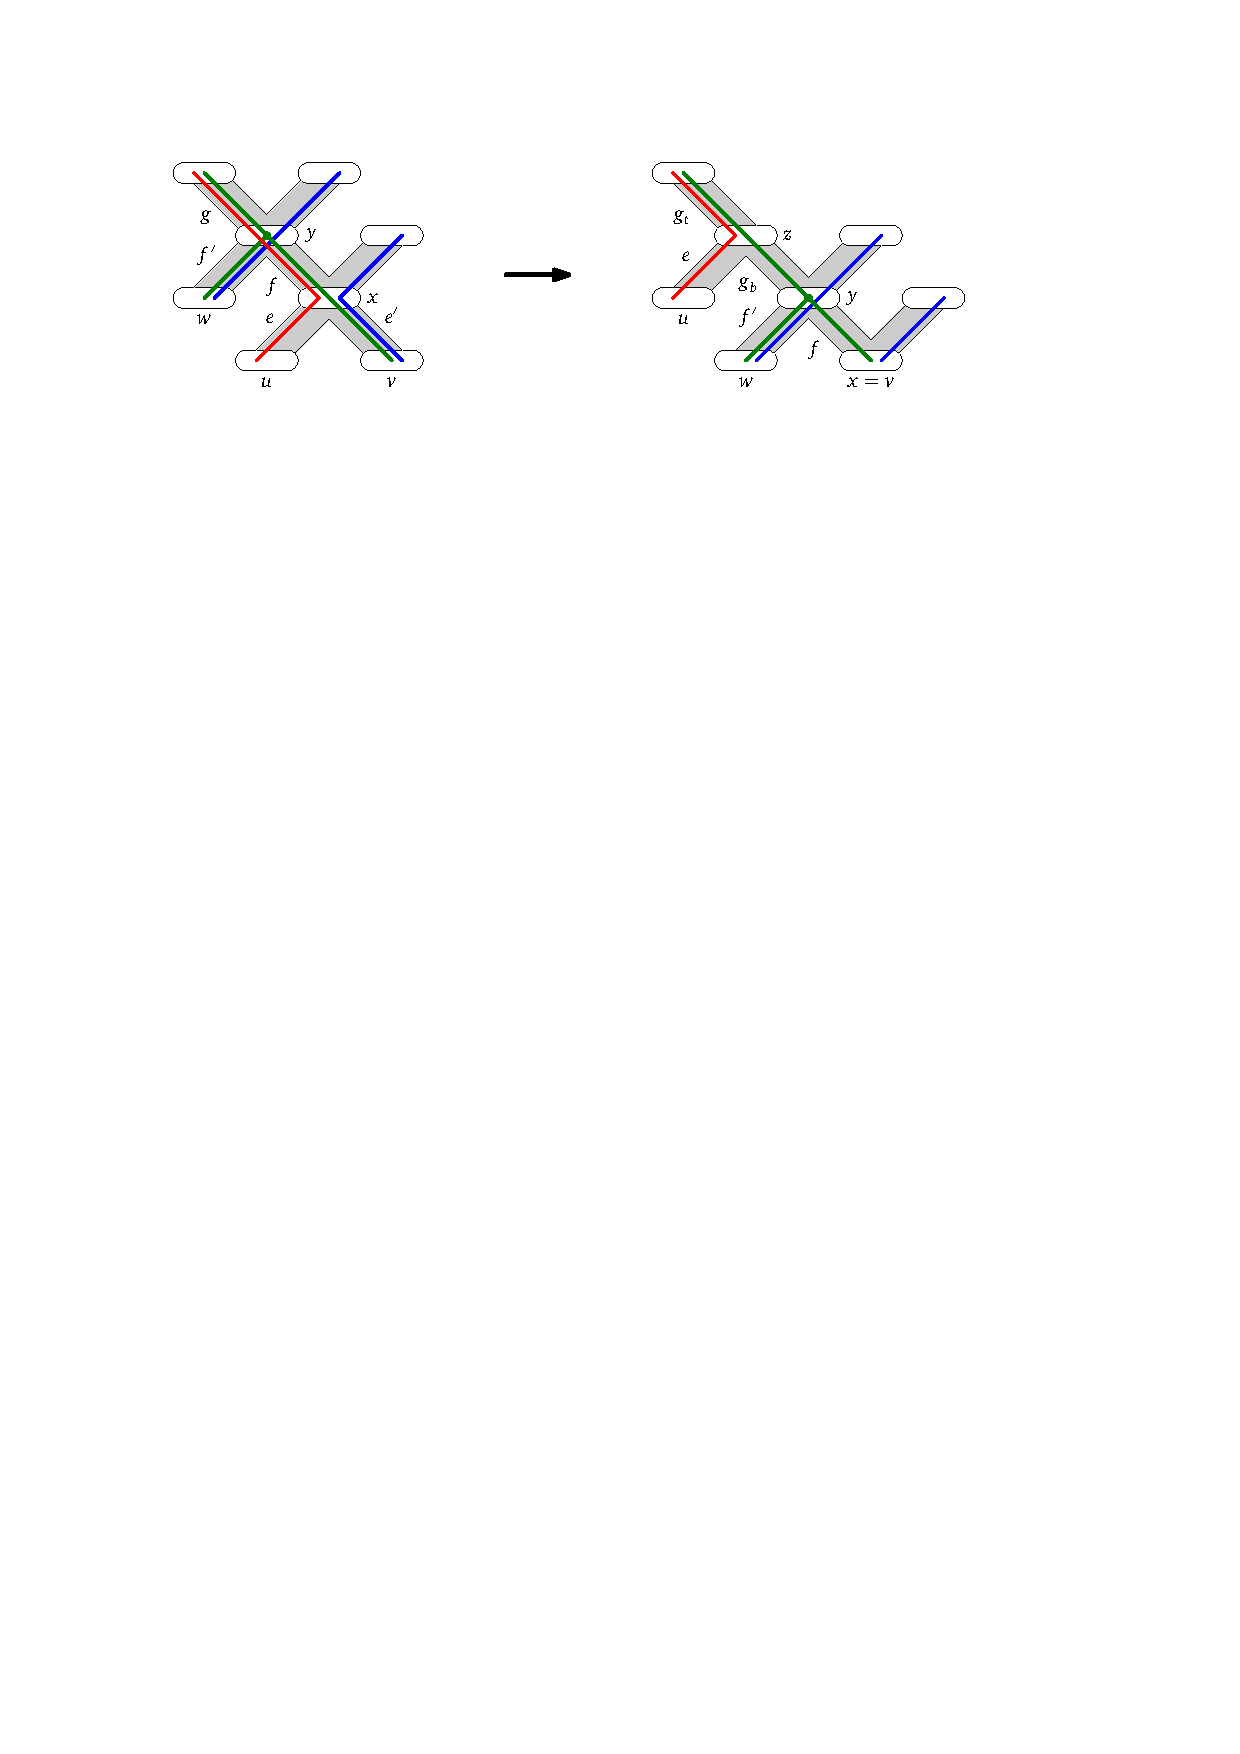
\includegraphics{../figs/ch4/foreign-split-transformation}
    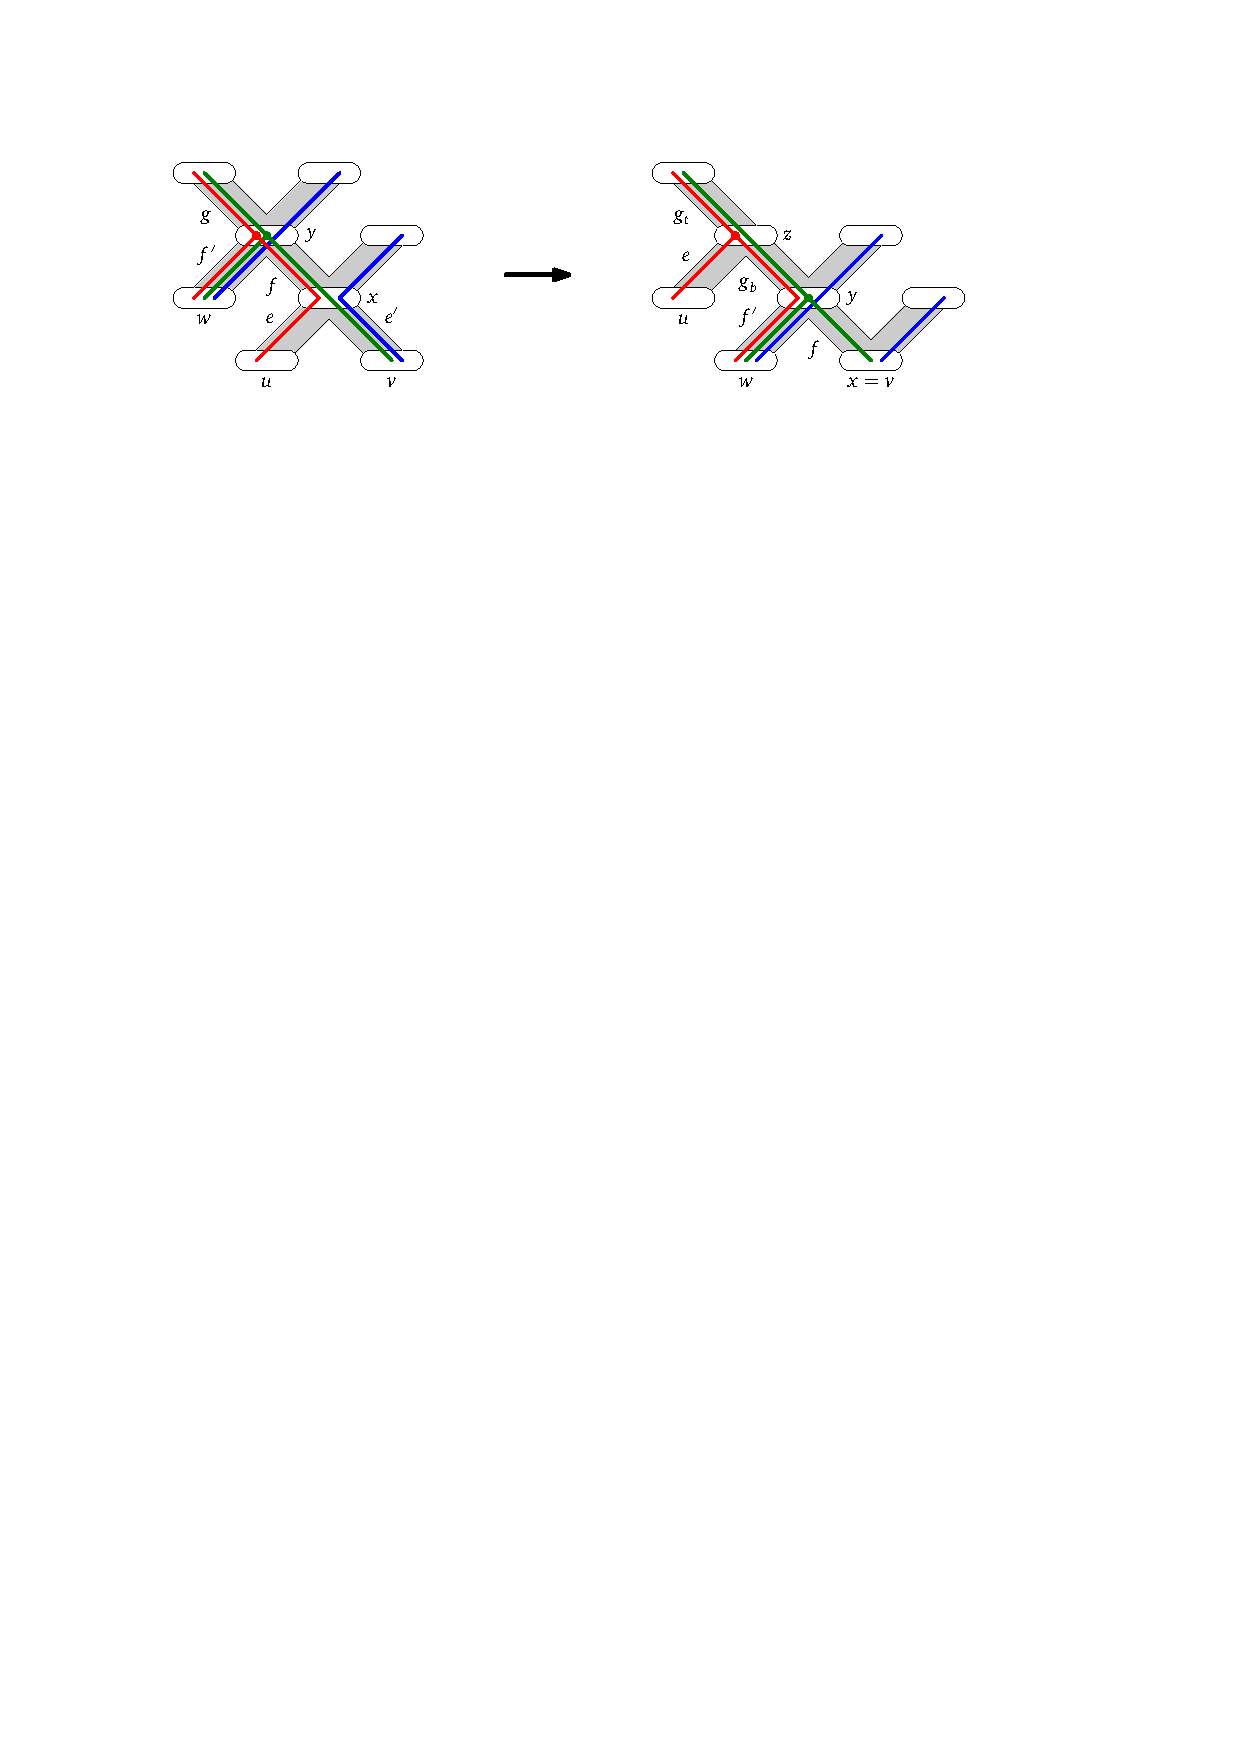
\includegraphics{../figs/ch4/double-split-transformation}
    \caption{Eliminating a fake split node $x$ below a split node $y$ {that is a~$T'$-split node with~$T'$ not equal to} the colour~$T$ {(red)} of the monochromatic edge below $x$.
      In the upper half of this figure $y$ is not a $T$-split node.
      In the lower half $y$ is a $T$-split node.}
    \label{fig:foreign-split-transformation}
  \end{figure}
  %-----------------------------------------------------------------------------

  If $y$ is a true split node, we distinguish two cases.   The first case is that~$y$ is a $T'$-split node, for some $T' \ne T$. This case is illustrated in Figure~\ref{fig:foreign-split-transformation}. Figure~\ref{fig:foreign-split-transformation}(a) depicts the subcase that~$y$ is not {also} a~$T$-split node while Figure~\ref{fig:foreign-split-transformation}(b) depicts the subcase that~$y$ is also a~$T$-split node. Both cases can be handled in a similar way.


  Let $g$ be the   parent edge of $y$ whose colour set includes $T$, and let $f'$ be $f$'s   sibling edge.   We subdivide $g$ into two edges $g_t$ and $g_b$, with $g_t$ above $g_b$, and   denote their common endpoint by $z$.   We remove $T$ from the colour set of $f$, set $C(g_t) := C(g)$ and $C(g_b) := C(g) \setminus \set{T}$ if $T\notin C(f')$ and $C(g_b) := C(g)$ if $T\in C(f')$, change the top endpoint of $e$   to $z$, remove all edges whose colour sets are now empty (this can only be $f$   and $g_b$), and finally restore Condition~\ref{cond:bifurcating-nodes}.   Again, it is easily verified that this does not introduce any violations of   conditions~\ref{cond:acyclic-network}--\ref{cond:no-useless-edges} and   does not increase the hybridization number of the network.   It also does not increase the potential of any node and eliminates $x$ from the network (because $x$ has only one child edge~$e'$ after changing $e$'s top endpoint and hence~$e'$ is being contracted).   The only new node is $z$.   If $T \in C(f')$, then $z$ is a true split node and its contribution to the network's potential is $0$.   Thus, since~$x$ is eliminated from the network, the network's potential decreases.   If $T \notin C(f')$, then $z$ is a fake split node.   However, its potential $\phi_z$ is less than $\phi_x$ {because for each path from the root to~$z$ in the modified network there is a corresponding path from the root to~$x$ in the original network that has bigger weight because it contains true split node~$y$.}   Thus, once again, the potential of the network decreases.

  %-----------------------------------------------------------------------------
  \begin{figure}
    \centering
    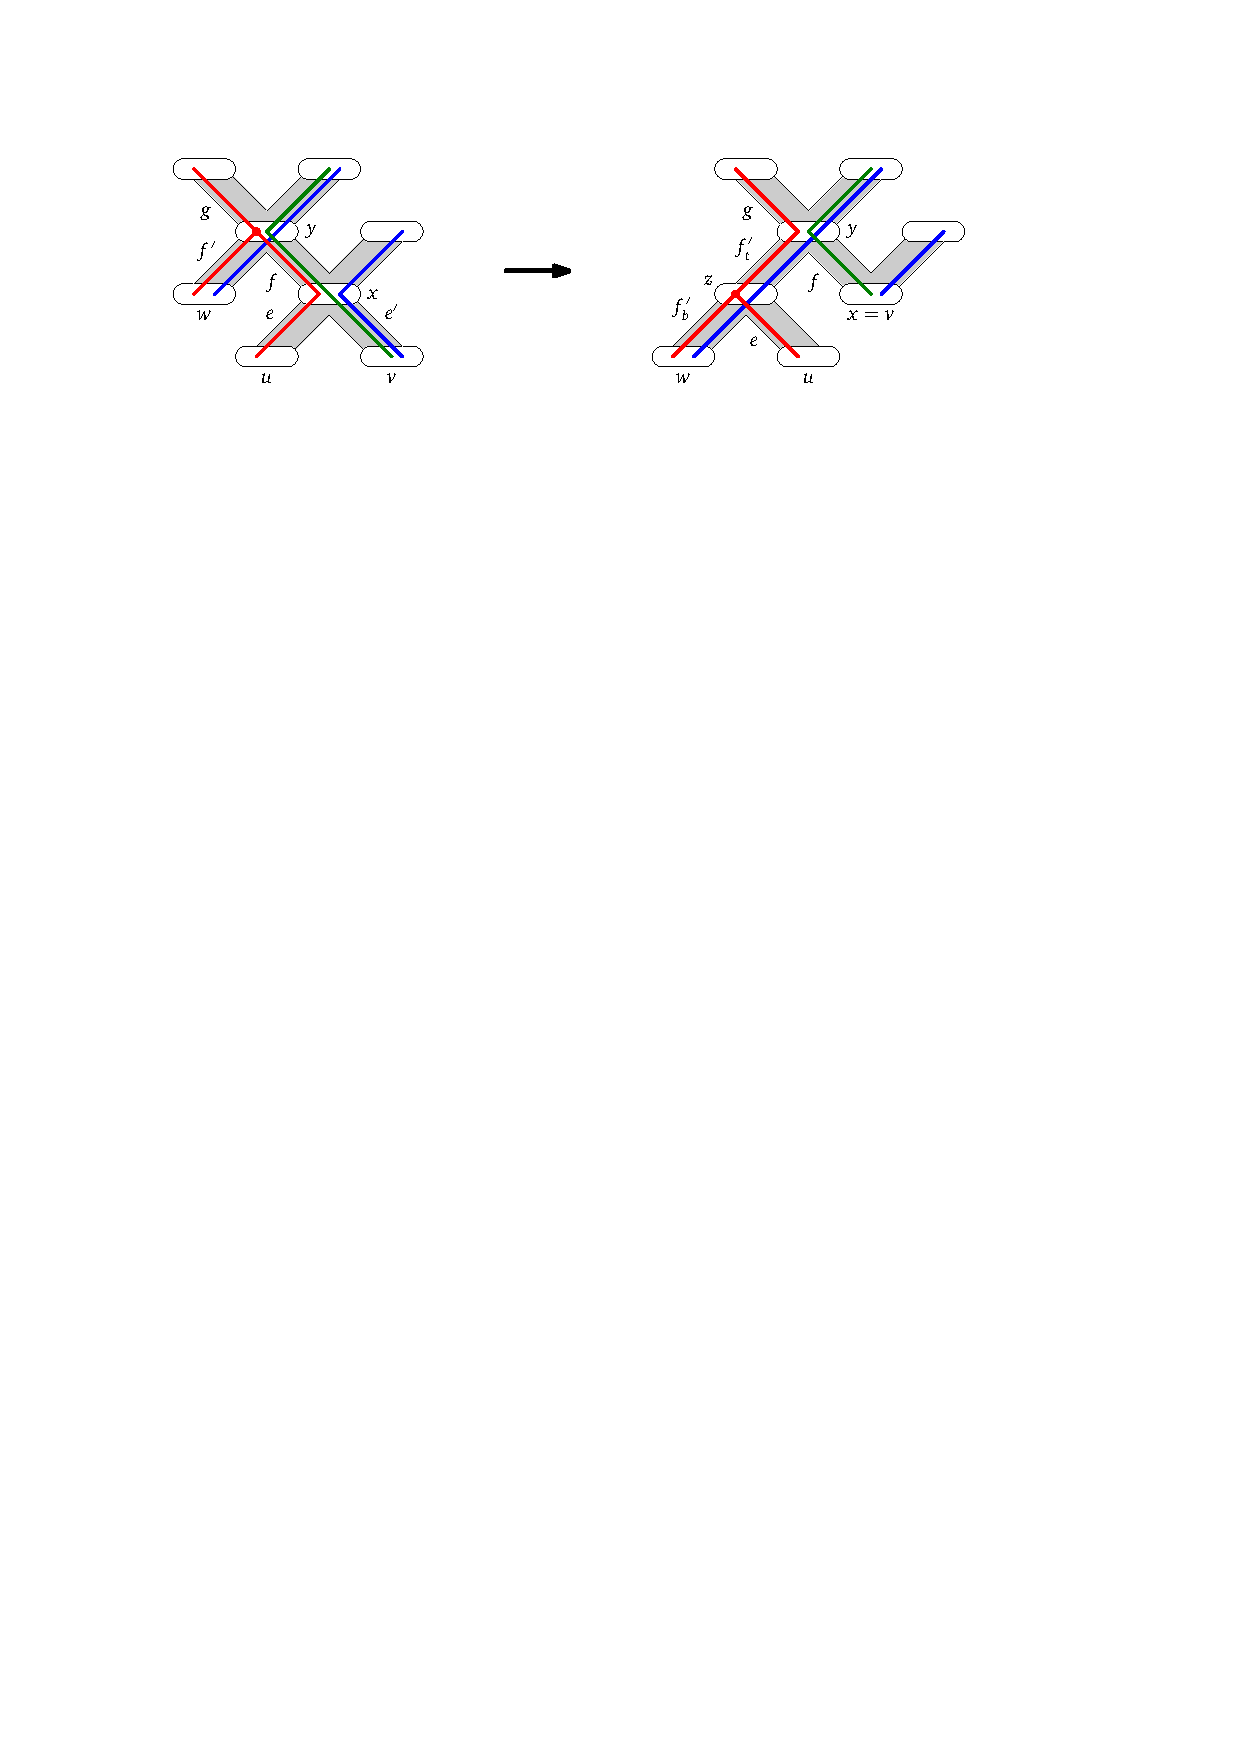
\includegraphics{../figs/ch4/self-split-transformation}
    \caption{Eliminating a fake split node~$x$ below a split node $y$ {that is not a~$T'$-split node for any~$T'$ that is not equal to the colour~$T$ (red) of the monochromatic edge below $x$.}}
    \label{fig:self-split-transformation}
  \end{figure}
  %-----------------------------------------------------------------------------

  Finally, if $y$ is not a $T'$-split node for any $T' \ne T$ (see   Figure~\ref{fig:self-split-transformation}), it must be a   $T$-split node. Let, as before, $g$ be the   parent edge of $y$ whose colour set includes $T$, and let $f'$ be $f$'s   sibling edge. We subdivide~$f'$ into~$f'_t$ and~$f'_b$ where~$f'_t$ is above~$f'_b$ and let~$z$ be the newly created node. Change the top endpoint of~$e$ to~$z$, remove~$T$ from the colour set of~$f$, remove all edges whose colour sets are now empty and restore Condition~\ref{cond:bifurcating-nodes}. This transformation maintains conditions   \ref{cond:acyclic-network}--~\ref{cond:no-useless-edges} and does not   increase the hybridization number of the network.   It eliminates fake split node $x$ from the network (because it has only one child edge~{$e'$} after   changing the top endpoint of~{$e$}) and makes~$y$ a fake split node.   However, the potential of~$y$ in the modified network is less than the potential of~$x$ in the original network. To see this, let~$P$ be a path of maximum weight from a root to~$y$. Then the potential of~$y$ in the modified network is one plus the weight of~$P$. In the original network, the path~$P$ extended by the edge~$(y,x)$ is then a path from a root to~$x$, and its weight is one higher than the weight of~$P$ {because it contains the true split node~$y$}. Hence, the potential of~$x$ in the original network is at least one higher than the potential of~$y$ in the modified network. Since the potential of all other nodes remains the same or decreases, the potential of the network decreases.
  
  Let $\H = (H', \E')$ be the CNET eventually obtained by the above transformations and let~$H$ be the original hybridization network. It remains to show that~$\H$ and~$H$ have the same deletion AAF. Observe that any node and edge of any component of the deletion AAF of~$H$ is contained in any embedding of each of the input trees. Using this observation, it can easily be checked that none of the modifications above alters the deletion AAF. In particular, the only case in the modifications for satisfying Condition~\ref{cond:every-node-splits} that involves an edge that is used by all three embeddings is the case depicted in Figure~\ref{fig:foreign-split-transformation}(b). Also the modification for this case does not alter the deletion AAF because the AAF component containing node~$w$ in the figure is not altered by the modification.
\end{proof}

By Lemma~\ref{lem:multiroot-is-fine}, it is sufficient if our algorithm can construct a CNET of the three input trees. In the next section, we show how to do this. 




%-------------------------------------------------------------------------------
\section{Reconstructing a canonical network}
%-------------------------------------------------------------------------------

\label{sec:guessing-things}

Let $\H = (H, \E)$ be a CNET for $\T$, let
$F$ be its deletion AAF, and let $k$ be its hybridization number.
For each tree $T \in \T$, let $I(T)$ be the set of nodes in $T$
that do not belong to any path between two leaves~$x$ and~$y$ in the same AAF
component (considering the root as a leaf).
In a sense, these nodes are ``invisible'' in $F$.
The \emph{extended AAF} $F^*$ of $\T$ is defined as
$F \cup I$, where $I := \bigcup_{T \in \T} I(T)$. {We will refer to the elements of~$F^*$ as \emph{components}. Let~$C$ be a component of~$F^*$. Hence,~$C$ is either an AAF component or a vertex in~$I$. If~$C$ is an AAF component, then~$r_C$ denotes the root of~$C$. If~$C$ is a vertex of~$I$, then~$r_C$ is equal to vertex~$C$. In either case, we will refer to~$r_C$ as the \emph{root} of component~$C$.}

By the following lemma, the size of~$I$ is at most~$3(k-1)$, when~$\T$ contains at most three trees.

\begin{lem}\label{lem:invisiblenodes}
For any~$T\in\T$, $|I(T)| \leq k-1$.
\end{lem}
\begin{proof}
Let~$T\in\T$. Since the root of~$T$ is a leaf after omitting directions, we can see~$T$ as an unrooted tree. Since~$F$ is an AAF of~$\T$ and~$T\in\T$, we know that~$F$ can be obtained by deleting a set~$E^*$ of~$k$ edges from~$T$ and then taking the partition of the leaves induced by the resulting connected components. Let~$\C$ be the partition of the vertices of~$I(T)$ induced by the connected components of the subgraph of~$T$ induced by~$I(T)$. For each~$C\in\C$, let~$\delta(C)$ denote the set of edges with exactly one endpoint in~$C$. Then, by the definition of~$I(T)$, at most one of the edges in~$\delta(C)$ is not contained in~$E^*$. Hence, from the~$|C|+2$ edges in~$\delta(C)$, at least~$|C|+1$ edges are in~$E^*$. Moreover, since~$T$ is a tree, at most~$|\C|-1$ edges can be in $\delta(C)\cap\delta(C')$ for two different~$C,C'\in\C$. Hence,
\[
|E^*| \geq \sum_{C\in\C} (|C|+1) - (|\C|-1) = |I(T)| + 1.
\]
Since~$|E^*|=k$, the lemma follows.
\end{proof}

We {will} construct $\H$ from $F^*$ and $\T$ with the help of a
\emph{guess} of the structure of $\H$.
In particular we construct $\H$ by ``gluing together'' the components
of $F^*$. Our guess concerns how this gluing is to be done.
The root $r_C$ of every component $C \in F^*$ has a unique image $H(r_C)$ in
$H$:
%%%%%%%%%%%
%\comment{NL}{I think it would be good to add a single sentence here saying what precisely $r_C$ can be (an actual root of a component or an invisible node). This is clear from the sentence above and also the definition of extended AAF, but I still found the notation slightly misleading.}\comment{LI}{I now explain this clearly after the definition of~$F^*$.}
%%%%%%%%%%%
If $C \in F$, this is true because $F$ is the deletion AAF of $\H$.
If $r_C = C \in I(T)$, for some $T \in \T$, $r_C$ is a split node of
{$T$ and, thus, has a unique image $H(r_C)$ in $H(T)$ which is also a node of~$H$}.
Our guess for $r_C$ defines the ``wiring'' of the in-edges of $H(r_C)$;
we call it the \emph{wiring guess} for $r_C$.
Since the colour sets of the parent edges of every node in $H$ are disjoint,
$H(r_C)$ has between one and three parent edges.
The first part of the wiring guess for $r_C$ is the number of parent edges of
$H(r_C)$.
The second part of the wiring guess for $r_C$ is which of these in-edges is
included in which tree image.
Finally, observe that the top endpoint~$x$ of each parent edge of~$H(r_C)$ must
once again be a $T'$-split node, for at least one $T' \in \T$.
%%%%%%%%%%
%\comment{NL}{I don't get this sentence. I thought this cannot be a T-split node of H for any T. I thought the top end point of parent egde of some $r_C$ is a reticulation, so that cannot be a tree node. I am most likely missing somehting.}\comment{LI}{but in a CNET each reticulation is also a split-node (or a leaf)}
%%%%%%%%%%
The third part of the wiring guess for $r_C$ determines such a tree $T'$ for
each parent edge of $H(r_C)$. {We will assume without loss of generality that any two nodes~$r_C,r_{C'}$ for which $H(r_C)$ and $H(r_{C'})$ have a common parent~$x$ both guess the same tree~$T'$ as the tree for which~$x$ is a~$T'$-split node.}

{First consider a component root~$r_C$ that is a vertex in~$I(T)$ for some~$T\in\T$.}
%%%%%%%%%%%
Note that (i) at least one parent edge of $H(r_C)$ must have colour $T$ because
$H(r_C)$ is {a non-root node} of $H(T)$, and (ii) the top endpoint
of a parent edge $e$ of $H(r_C)$ can be a $T'$-split node only for trees $T'$
such that $T' \in C(e)$.
%\comment{NL}{I guess the small case c in $r_c$ is a typo.} Leo: fixed it
%%%%%%%%%%%
This gives the~$17$ possible wiring guesses for~$r(C)$ shown in Figure~\ref{fig:guesses}.

If $r_C$ is an AAF root, the set of possible wiring guesses is more restricted.
Since $H(r_C)$ is contained in every tree image, the only valid wiring guesses
are the ones where the union of the colour sets of the parent edges of $H(r_C)$
contains all three colours. This reduces the number of possible wiring guesses for AAF roots to $10$ {(see again Figure~\ref{fig:guesses})}. {Finally note that, when~$r_C$ is the root~$\rho$ of the trees, there is only a single wiring guess.}

Our \emph{guess} $\G$ of the structure of $\H$ consists of the wiring guesses for all roots $r_C$, $C \in F^*$.

%-------------------------------------------------------------------------------
\begin{figure}
  \centering
  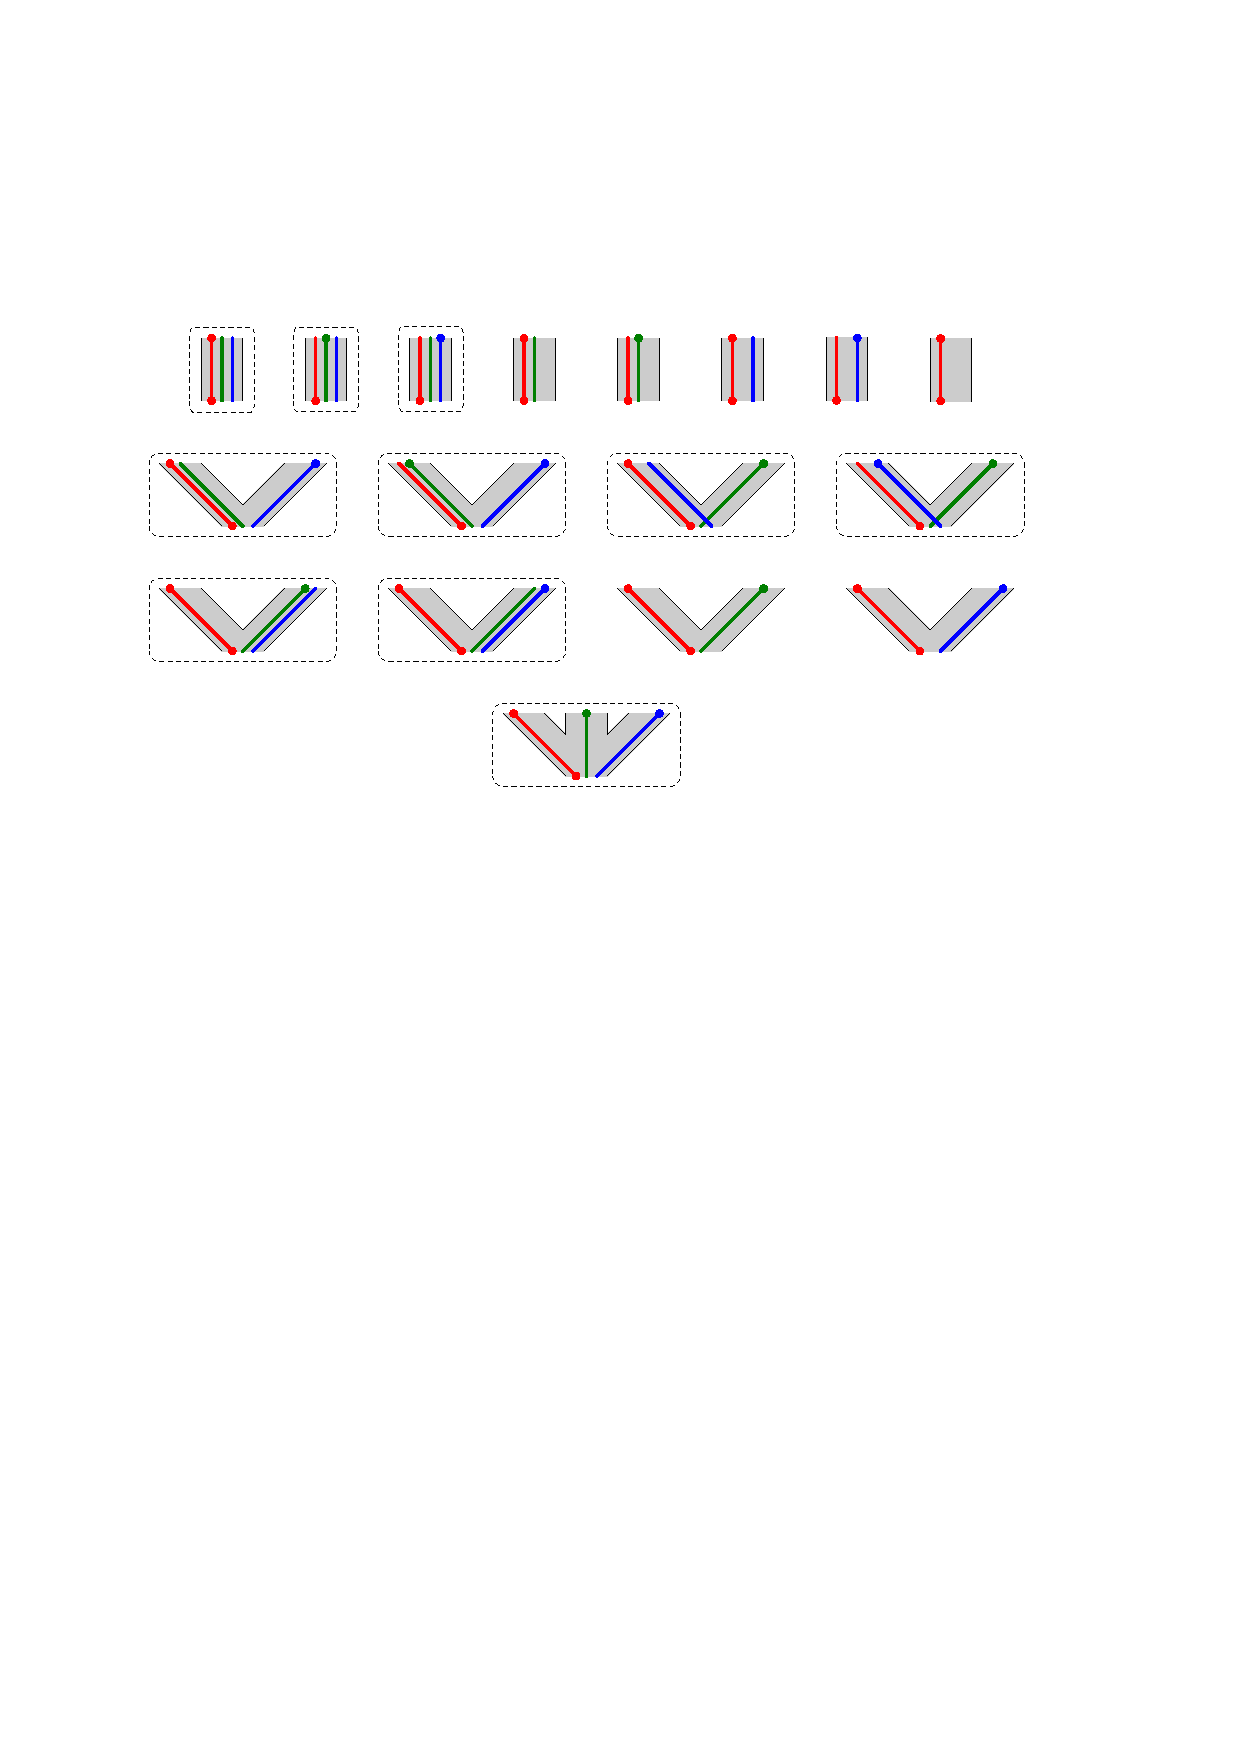
\includegraphics{../figs/ch4/guesses}
  \caption{The 17 possible wiring guesses for {the root~$r_C$ of a component~$C$ of the extended AAF~$F^*$ that is a node in~$I(T)$, with~$T$ the red tree}.
    The guess of the split node at the top of each edge is indicated by a dot.
    Valid guesses for a root~$r_C$ of an AAF component are indicated by dashed boxes around them.}
  \label{fig:guesses}
\end{figure}
%-------------------------------------------------------------------------------

Since we have $17$ wiring guesses to choose from for each component in $I$,
and $10$ wiring guesses to choose from for each component in $F$ that does not
contain the tree root $\rho$, there are $10^{\size{F}-1} \cdot 17^{\size{I}}$
possible guesses $\G$.
Since $\size{F} \le k+1$ and $\size{I} \le 3(k-1)$ by Lemma~\ref{lem:invisiblenodes}, the number of possible guesses $\G$ is bounded
by $10^k \cdot 17^{3(k-1)} = 49130^k / 4913$.

Our algorithm considers each guess {in}~$\G$ in turn and attempts to construct a
CNET $\H$ from $(\G, F^*, \T)$ in polynomial time.
We call $(\G, F^*, \T)$ the CNET's \emph{description}.
To establish our algorithm's correctness, we prove that, given the description
$(\G, F^*, \T)$ of a CNET $\H$ for $\T$, our
algorithm succeeds in constructing a CNET $\H'$ for
$\T$ with description $(\G, F^*, \T)$ that differs from $\H$ only in
insignificant details and in particular has the same hybridization number
as~$\H$. Our proof is divided into two lemmas. The first one shows that two CNETs with the same description are essentially
the same.
We make this precise below.
The second one shows that, given the description of a CNET, we can construct a CNET with this description in polynomial time.
Note that not every description $(\G, F^*, \T)$ is necessarily a valid
description of any CNET.
{If there is no CNET with the given description, then our algorithm will determine this polynomial time.} The description of this algorithm is given in the proofs of
Lemmas~\ref{lem:unique-network} and~\ref{lem:network-from-description} below.
Appendix~\ref{sec:example} provides an example of the operation of the
algorithm.

Given a CNET $\H = (H, \E)$ for $\T$, we obtain a DAG $\tilde H$ by contracting the image of every component of the deletion AAF $F$ of $H$ into a single node, keeping parallel edges this creates. We call $\tilde H$ the \emph{signature} of $H$. {For an example, see Figure~\ref{fig:reconstruction-signature} in the appendix.} It is easy to see that the node set of $\tilde H$ is $\set{H(r_C) \mid C \in F^*}$ and that $\tilde H$ has the same hybridization number as $H$. Note that two nodes~$C\in I(T)$, $C'\in I(T')$ might map to the same node~$H(r_C)=H(r{_C'})$ of~$\tilde H$. We label every node $x$ of $\tilde H$ with the set of roots $r_C$, $C \in F^*$, such that $x = H(r_C)$. We call roots that label the same node of~$\tilde H$ \emph{buddies} (of each other). Note that roots of components of~$F$ have no buddies. We call two CNETs $\H = (H, \E)$ and $\H' = (H', \E')$ \emph{equivalent} if $\tilde H = \tilde H'$. In particular, two equivalent CNETs have the same hybridization number. 

{Before proving that CNETs with the same description are always equivalent, we introduce two useful notions which we will use in the two upcoming proofs.}

We will use the following notion of the {``attached subtrees''} of an AAF component~$C$ in a tree~$T$. For each edge~$(u,v)$ of~$T$ for which~$u$ is contained in~$T(C)$ but~$v$ is not contained in~$T(C)$, we say that the subtree of~$T$ induced by~$u,v$ and all nodes reachable from~$v$ is {a subtree of~$T$ \emph{attached} to~$C$.}
  
In addition, we will use the following notion of the ``pendant subtrees'' represented by an edge~{$e=(r_C,r_{C'})$ of the signature~$\tilde H$. For each~$T\in C(e)$, the subtree of~$T$ induced by~$r_{C'}$, the parent of~$r_{C'}$ and all vertices reachable from~$r_{C'}$ is} said to be a \emph{pendant subtree} of~$T$ represented by the edge~$e$ of~$\tilde H$.

%-------------------------------------------------------------------------------
\begin{lem}
  \label{lem:unique-network}
  If two CNETs have the same description, then they are equivalent.\footnote{The reverse statement does not hold.}
\end{lem}
%-------------------------------------------------------------------------------

\begin{proof}
  Given the description $(\G, F^*, \T)$ of a CNET
  $\H = (H, \E)$, we show how to uniquely reconstruct $\tilde H$ from this
  description.
  We define a DAG $D$ whose nodes are the roots of {components of}~$F^*$.
  There is an edge from a root $r_C$ to a root $r_{C'}$ if and only if there
  exists a tree $T \in \T$ such that $r_{C'}$ is an ancestor of $r_C$ in $T$
  and there exists no component root $r_{C''}$ that is an ancestor of $r_C$ and
  a descendant of $r_{C'}$ in~$T$.
  If this is the case, we call $r_C$ a \emph{direct descendant} of $r_{C'}$ in $T$.
  We incrementally construct a topological ordering of $D$, define $U_i$ to be the first~$i$ nodes in this topological ordering, $D_i$ to
  be the subgraph of $D$ induced by $U_i$ and $V_i := \{ H(r_C) \mid r_C \in U_i\}$.
  $\bar D_i$~is the subgraph of $D$ induced by all nodes of $D$ not in $U_i$. Let {the partial signature} $\tilde H_i$ be the graph obtained from the subgraph of $\tilde H$ induced by~$V_i$ by, for each parent edge~$e$ in~$\tilde H$ of a node $H(r_C) \in V_i$ whose top endpoint does not belong to $V_i$, adding a new root with an edge~$\tilde e$ from this new root to~$H(r_C)$ and giving~$\tilde e$ the same colour set as~$e$ (which is determined by the set of guesses). {For an example, see Figure~\ref{fig:reconstruction-signature} in the appendix.} We will call an edge whose top endpoint is a root a \emph{root edge}.
	
%	\comment{NL}{I thought that using words ``partial signature'' or something like this to refer to $\tilde H$ would clarify this paragraph a bit.} Leo: done.
  
%  In addition, for every node $H(r_C) \in V_i$, $\tilde H_i$ contains a parent
%  edge $\tilde e$ corresponding to each parent edge $e$ of $H(r_C)$ in
%  $\tilde H$ whose top endpoint does not belong to $V_i$.
%  Edges $e$ and $\tilde e$ have the same colour set, but the top endpoint of
%  $\tilde e$ is a root of $\tilde H_i$ with a single child even if the top
%  endpoint of $e$ is not a root of $\tilde H$.

  We assign these new roots colours, where the colour of the top endpoint
  of edge $\tilde e$ is $T$ if the bottom endpoint of $\tilde e$ guesses that the top endpoint of $e$ is a $T$-split node.
  
We will show that, from~$D_i, \tilde H_i$ and~$\G$, we can determine a unique nonempty set of nodes~$U'$ of $\bar D_i$, the set~$U^+$ of all buddies of nodes in~$U'$ and {an extended partial signature}~$\tilde H_j$ corresponding to the graph~$D_j$ induced by~$U_j:=U_i\cup U' \cup U^+$.
  
%  We show that $D_i$ defines a unique non-empty set of nodes in $\bar D_i$ such
%  that the set of buddies of each such node $r_C$ in $\tilde H$,
%  along with the graph $\tilde H_j$ corresponding to the graph
%  $D_j \supset D_i$ obtained by adding $r_C$ and all its buddies to $D_i$,
%  can be determined from $\tilde H_i$ and $\G$.
  
%  We choose such a node $r_C$, add all its buddies to $D_i$, and augment
%  $\tilde H_i$ to obtain the graph $\tilde H_j$ corresponding to the resulting
%  graph $D_j \supset D_i$.
  
  Once $D_i = D$, we thus obtain $\tilde H_i = \tilde H$, that is, we are able
  to reconstruct {the signature} $\tilde H$ only given the description of~$\H$.
  
We initialize the reconstruction by defining $D_0$ and~$\tilde H_0$ to be empty {digraphs}. Now consider an iteration with input {digraph} $D_i$ and {partial signature} $\tilde H_i$. 
%   such that
%  $H(r_C) \in \tilde H_i$ if and only if $r_C \in D_i$.
  For an in-degree-$0$ node $r_C$ of $\bar D_i$ that belongs to $I(T)$, for some
  $T \in \T$, observe that both child edges of $H(r_C)$ in $\tilde H$ have corresponding root edges in $\tilde H_i$ (by the construction of $\tilde H_i$). For such a node~$r_C$, we call $r_C$ \emph{free} if the top endpoints of both of these root edges are coloured $T$.
  For an in-degree-$0$ node $r_C$ of $\bar D_i$ that is a root of {a component of} $F$, we say that~$r_C$ is \emph{free}
  if, for every in-edge $e$ of $r_C$ in $D$, the corresponding root edge $\tilde e$ of $\tilde H_i$ has the property that, for every
  $T \in C(\tilde e)$, the {pendant} subtree of $T$ represented by $\tilde e$ is {attached to the AAF component $C$ in $T$}. All other nodes of $\bar D_i$ are non-free.
  We claim that at least one of the nodes in $\bar D_i$ is free and that every
  free node can determine its buddies in $\tilde H$ and can augment {the partial signature} $\tilde H_i$
  to $\tilde H_j$.

  Consider a node $x$ of {the signature} $\tilde H$ that does not belong to $\tilde H_i$ and all of whose children {do} belong to $\tilde H_i$.
  Since $\tilde H$ is a DAG, such a node exists.
  Node $x$ is a $T$-split node, for some $T \in \T$, and is thus the image
  $H(r_C)$ of {the root~$r_C$ of a component} in~$F \cup I(T)$.
  
  First consider the case that {$C \in F$}. Observe that, because $\tilde H$ is the signature of a CNET $\H$ for $\T$, the {subtrees attached to} $C$ in all input trees are exactly the {pendant} subtrees represented by the child
edges of $H(r_C)$ in $\tilde H$. Since these child edges are root edges of $\tilde H_i$, $r_C$ is free. Node $r_C$ can trivially identify its set of buddies because it has no buddies besides itself. We obtain~$D_j$ by adding $r_C$ to $D_i$ and obtain~$\tilde H_j$ from~$\tilde H_i$ by locating the root edges of $\tilde H_i$ that correspond to child edges of $H(r_C)$ in $\tilde H$, merging the top endpoints of these root edges to a single node~$H(r_C)$, and adding new root edges entering~$H(r_C)$ according to~$r_C$'s wiring guess.
%  We add $r_C$ to $D_i$ and augment $\tilde H_i$ by identifying the top
%  endpoints of all root edges that represent child edges of $H(r_C)$ in
%  $\tilde H$ with each other and adding parent edges to the resulting node
%  according to $r_C$'s wiring guess.
  This gives a new graph $D_j \supset D_i$ and the corresponding graph
  $\tilde H_j$.

  Now consider the case that $r_C \in I(T)$. In this case, both child edges of~$r_C$ in $\tilde H$ correspond to root edges of $\tilde H_i$.
  Since these two edges have a common top endpoint in $\tilde H$, their
  top endpoints in $\tilde H_i$ must have the same colour $T'$.
  This implies that $H(r_C)$ is a $T'$-split node and is thus the image
  $H(r_{C'})$ of a node $r_{C'} \in I(T')$.
  Since the child edges of $H(r_{C'})$ in~$\tilde H$ belong to $\tilde H_i$, both
  in-neighbours of $r_{C'}$ in $D$ belong to $D_i$.
  Thus, $r_{C'}$ is free.
  Since $H(r_C) = H(r_{C'})$, we may assume that $r_{C'} = r_C$ (because in at least one set of guesses this is the case). We obtain $\tilde H_j$ from~$\tilde H_i$ by locating the two root edges of~$\tilde H_i$ that correspond to child edges of $H(r_C)$ in $\tilde H$, merging the top endpoints of these edges to a single node~$H(r_C)$, and adding new root edges entering~$H(r_C)$ according to~$r_C$'s wiring guess.
%  We obtain $\tilde H_j$ by identifying the top endpoints of the two child
%  edges of $H(r_C)$ in $\tilde H_i$ with each other and adding parent edges to
%  the resulting node according to $r_C$'s wiring guess.
  Now consider the child edges of $H(r_C)$ in $\tilde H_j$.
  For each tree $T' \in \T$ such that these edges are both coloured $T'$,
  $H(r_C)$ is the image $H(r_{C'})$ of a node in $I(T')$.
  The nodes of $\bar D_i$ that satisfy this condition are the buddies of
  $r_C$, and we add them to $D_i$ along with $r_C$ to obtain $D_j$.

  We have shown that every node $H(r_C)$ of $\tilde H$ whose children belong to
  $\tilde H_i$ corresponds to a free node $r_C$ in $\bar D_i$ and that $r_C$
  can determine its set of buddies and can construct the {extended partial signature} $\tilde H_j$
  corresponding to the {digraph} $D_j \supset D_i$ obtained by adding these buddies to $D_i$.
  If $r_C$ is an AAF root, it has no buddies besides itself.
  If $r_C \in I(T)$, for some $T \in \T$, observe that none of its buddies is
  free because it belongs to a tree $T' \ne T$ but the top endpoints of the
  child edges of $H(r_C)$ have colour $T$ in $\tilde H_i$.
  Thus, to prove that \emph{every} free node can determine its set of buddies
  and can construct $\tilde H_j$ from $\tilde H_i$, it suffices to show
  that there is no free node $r_C$ such that $H(r_C)$ has an in-neighbour not in
  $\tilde H_i$.

  Assume there exists such a node $r_C$.
  {Then} $r_C$ has in-degree $0$ in $\bar D_i$ because otherwise it
  is not free.
  First assume $r_C$ {is the root of a component} in~$F$.
  Let $H(r_{C'})$ be an in-neighbour of $H(r_C)$ in $\tilde H$ that does not
  belong to~$\tilde H_i$, and let $T$ be an arbitrary colour $T$ in the
  colour set of the edge $e$ between $H(r_C)$ and $H(r_{C'})$ in~$\tilde H$.
  Since $r_C$ has in-degree~$0$ {in $\bar D_i$}, the {pendant} subtree of $T$ represented by $e$ is also represented by some root edge $f$ of $\tilde H_i$.
  Thus, $\tilde H$ contains a unique path from $e$ to $f$ and every node on this
  path is a $T'$-split node, for some $T' \ne T$.
  This implies in particular that the top endpoint of edge $f$ is a $T'$-split
  node, {$T,T'\in C(f)$}, and the {pendant} subtree of $T'$ represented by $f$ is not a {subtree attached to $C$ in~$T'$}. Thus, since $f$ represents the same in-edge of $r_C$ in $D$ as $e$, $r_C$
  is not free, a contradiction.

  If $r_C \in I(T)$, for some tree $T \in \T$, we choose an in-neighbour
  $H(r_{C'})$ and a root edge $f$ of $\tilde H_i$ as in the case when
  $r_c \in F$.
  Since the top endpoint of edge $f$ is not a $T$-split node, its colour in
  $\tilde H_i$ must be $T' \ne T$.
  Thus, since $f$ is the root edge of $\tilde H_i$ representing one of the
  in-edges of $r_C$ in $D$, $r_C$ is not free, again a contradiction.
\end{proof}

By Lemma~\ref{lem:unique-network}, it suffices to provide a polynomial-time
algorithm that decides whether there exists a CNET
with description $(\G, F^*, \T)$ and, if so, construct any such CNET.
Our next lemma states that such an algorithm exists.

%-------------------------------------------------------------------------------
\begin{lem}
  \label{lem:network-from-description}
  Given a description $(\G, F^*, \T)$, it takes polynomial time to decide
  whether there exists a CNET with this description
  and, if so, {to} construct such a CNET.
\end{lem}
%-------------------------------------------------------------------------------

\begin{proof}
  The proof of Lemma~\ref{lem:unique-network} already specifies an algorithm
  for constructing the signature $\tilde H$ of a CNET $\H = (H, \E)$ with
  description $(\G, F^*, \T)$, if such a CNET exists, and this algorithm is
  clearly implementable in polynomial time.
  This algorithm provides a first test that can be used to reject invalid
  descriptions:
  If the algorithm reaches an iteration where $\bar D_i$ is non-empty but none   of its nodes is free, then the description is invalid because   the proof of Lemma~\ref{lem:unique-network} shows that, if $(\G, F^*, \T)$   is the description of a CNET, then there exists   a free node in each iteration.   Thus, the algorithm aborts and rejects the description.   If the algorithm does not reject the description, its output is a signature   $\tilde H$ that respects all wiring guesses in $\G$.   However, this signature may not correspond to a network $H$ that displays   all input trees.   Next we present a polynomial-time algorithm for constructing $\H = (H, \E)$   from $\tilde H$, $F^*$, and $\T$ or determining that no CNET $\H = (H, \E)$   with description $(\G, F^*, \T)$ exists.

  The nodes of $\tilde H$ are of two types: images of AAF roots and images of   {nodes in~$I$.}   To obtain a CNET $\H = (H, \E)$ with description $(\G, F^*, \T)$ from   $\tilde H$, {we let~$H$ initally be equal to~$\tilde H$ and will} replace each AAF root image with the AAF component it represents.   We process these AAF root images bottom-up, that is, in reverse topological   order.\footnote{This is not really essential, but it simplifies the     description of the algorithm.}   Consider such an image $H(r_C)$ of the root $r_C$ of an AAF component $C$, and   let $E$ be the set of child edges of $H(r_C)$ in $\tilde H$.   We remove the edges in $E$ from $\tilde H$ and attach $C$ below $r_C$, setting   $C(e) = \T$ for every edge $e$ of $C$.   Our goal now is to reattach the edges in $E$ to edges of $C$ so that, for all   $T \in \T$, the descendant edges of $H(r_C)$ with colour $T$ form an image   of the {pendant subtree of~$T$ with root~$r_C$}.   For each tree $T$, observe that the edges in $E$ coloured $T$ represent the  {subtrees attached to} $C$ in $T$.   We need to attach these edges to $C$ {in~$H$} so that each edge branches off the same edge of $C$ as in $T$ and edges that branch off the same edge of $C$ in $T$ do so in the same order as in $T$.

  First we test every edge $e \in E$ whether $e$ branches off the same edge of $C$ in every tree {$T\in C(e)$}.   If this is the case for all edges $e \in E$, then we can partition $E$ into   subsets $E_f$, one per edge $f$ of $C$, such that all edges in $E_f$ branch   off edge $f$.   If there is an edge $e$ that branches off some edge $f$ in a tree $T \in C(e)$   and off a different edge $f'$ in a tree $T' \in C(e)$, it is impossible to   attach this edge to $C$ in a way that satisfies both constraints.   Since the edges of $T$ and $T'$ represented by $e$ are determined by   $\tilde H$,   which in turn is uniquely defined by $(\G, F^*, \T)$, there is thus no network   $\H$ with description $(\G, F^*, \T)$, so the algorithm aborts and reports   that there is no such network. 

  Given the partition of $E$ into subsets $E_f$ such that the edges in $E_f$   branch off edge $f$, we need to attach the edges in each such set $E_f$   in an ordering consistent with the input trees.   Let $E_{f,T}$ be the subset of edges in $E_f$ that have colour $T$.   Tree $T$ determines the ordering in which these edges need to be attached to   $f$. We define a DAG $D_f$ whose nodes represent the edges in $E_f$, and {which has an edge~$(g,g')$ precisely if there is a tree~$T$ such that~$g,g'\in E_{f,T}$ and~$g$ branches off~$f$ in~$T$ above~$g'$.}   There exists an ordering in which to attach {the edges of~$E_f$} to $f$ so that   the ordering constraints imposed by all trees in $\T$ are satisfied if and   only if $D_f$ is acyclic. {Moreover, if~$D_f$ is indeed acyclic, then a topological ordering of $D_f$ provides a valid ordering in which the edges can be attached.}   Thus, we can test whether such an ordering exists and, if so, compute such   an ordering in time $\Oh(\size{E_f})$ per edge $f$.   If no such ordering exists, the algorithm once again aborts and reports that   there is no CNET with description $(\G, F^*, \T)$.   If we can find a correct ordering of the edges attached to each edge $f$   of $C$, then the replacement of $r_C$ with $C$ in this manner results in   a network where all descendant edges of $H(r_C)$ with colour $T$ form   an image of {the pendant subtree of~$T$ with root~$r_C$}, for all $T \in \T$.   Thus, after replacing each AAF root $r_C$ with its corresponding component   $C$ in this fashion, we obtain a CNET $\H = (H, \E)$ with   description $(\G, F^*, \T)$.
\end{proof}


%-------------------------------------------------------------------------------
\section{An Example of constructing a network from its description}
%-------------------------------------------------------------------------------

\label{sec:example}

This appendix provides an example of the construction described in the proofs of
Lemmas~\ref{lem:unique-network} and~\ref{lem:network-from-description}.
Consider the description $(\G, F^*, \T)$ in
Figure~\ref{fig:reconstruction-input}.
The CNET in Figure~\ref{fig:reconstruction-output} has this description.
We first show how to construct its signature using the construction in the
proof of Lemma~\ref{lem:unique-network}.
This signature is shown in Figure~\ref{fig:reconstruction-signature}.
Then we discuss how to construct the CNET in
Figure~\ref{fig:reconstruction-output} from this signature.
{The hybridization network induced by this CNET} is shown in Figure~\ref{fig:reconstruction-final}.

%-------------------------------------------------------------------------------
\begin{figure}[h]
  \centering
  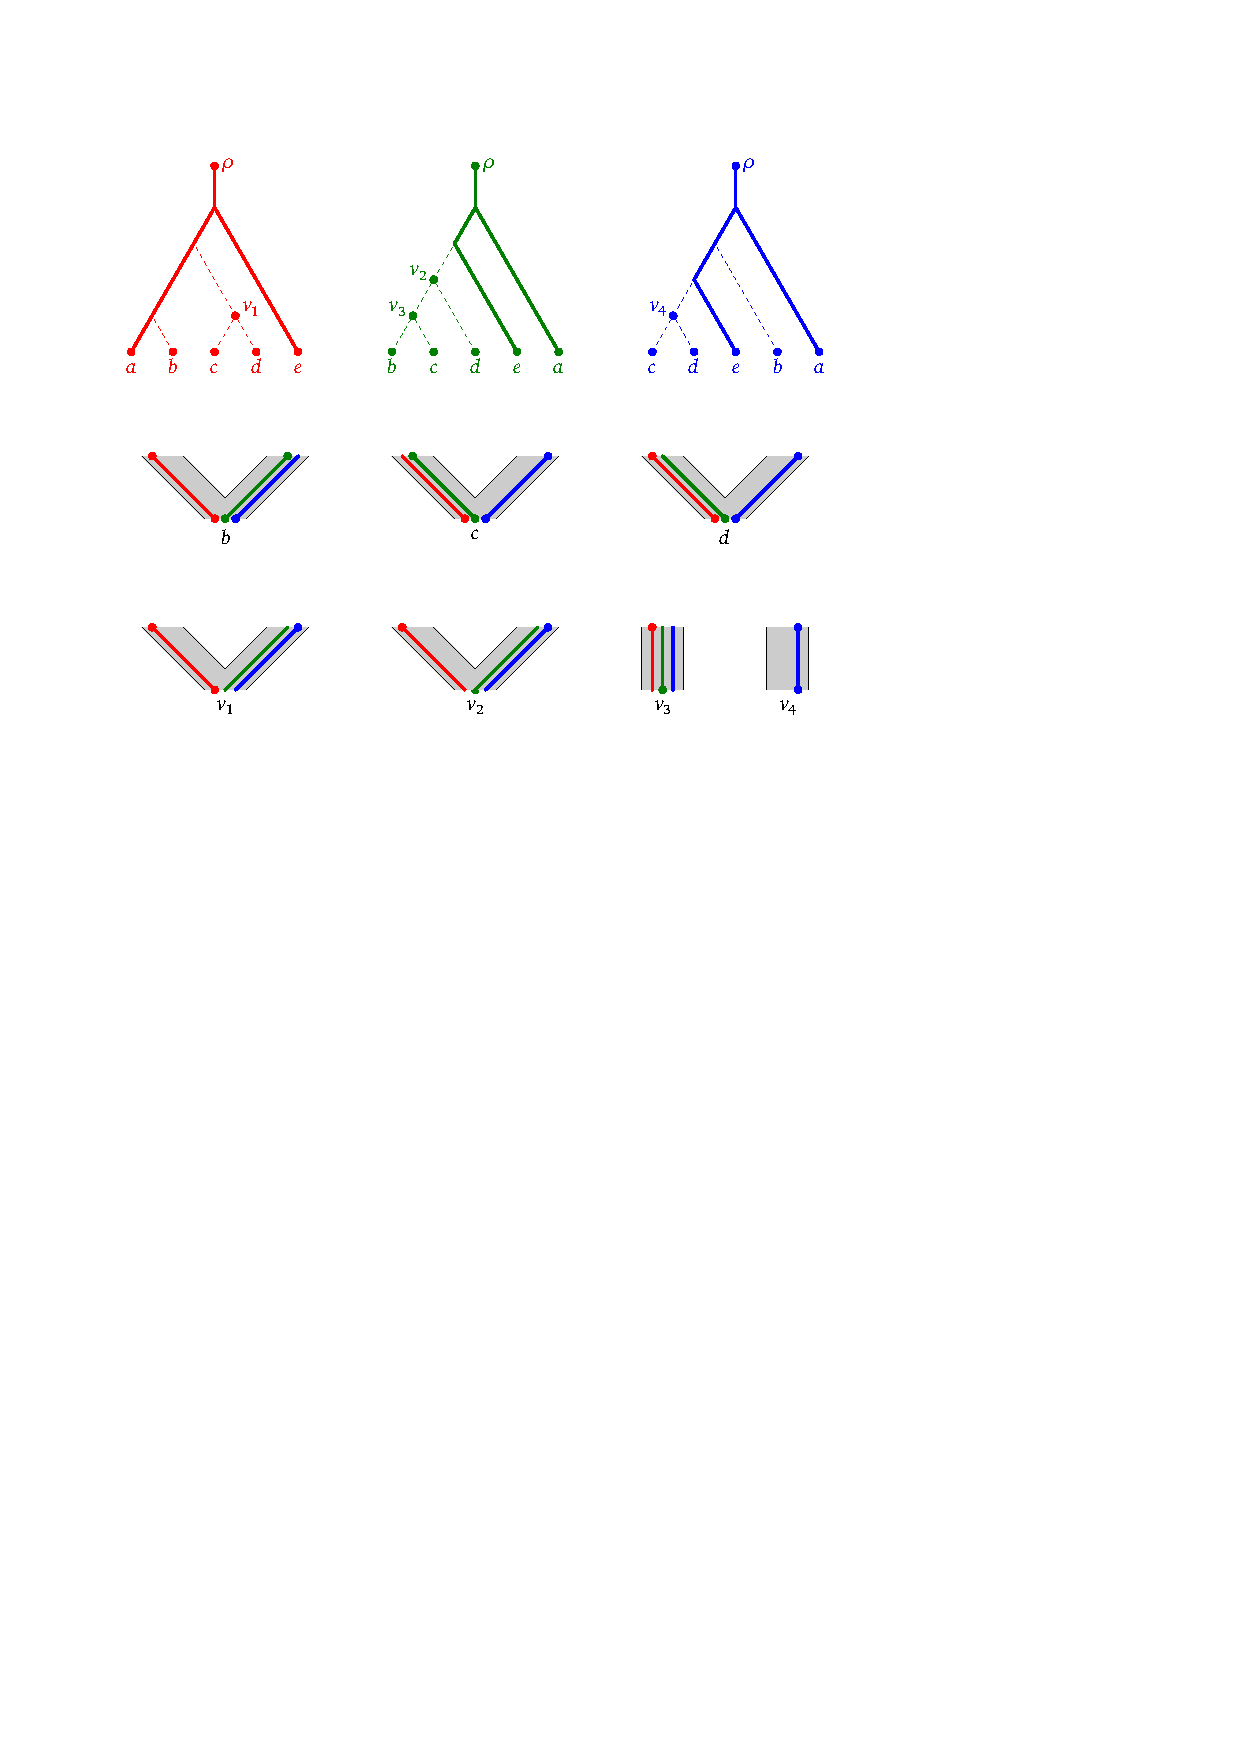
\includegraphics{../figs/ch4/reconstruction-input-trees}
  \caption{The input to the network reconstruction, including the AAF $F$ (shown
    in bold in the three input trees), {the set of ``invisible nodes'' $I=\{v_1,\ldots ,v_4\}$}, and the wiring guesses
    for the resulting set of components of $F^*$. There is no guess for the component $\set{a, e, \rho}$ because it includes
    the root~{$\rho$} of the three trees.}
  \label{fig:reconstruction-input}
\end{figure}
%-------------------------------------------------------------------------------

%-------------------------------------------------------------------------------
\paragraph{Lemma~\ref{lem:unique-network}: Constructing the signature.}
%-------------------------------------------------------------------------------

The DAG $D$ used in the construction of the signature $\tilde H$ of any CNET
with the description in Figure~\ref{fig:reconstruction-input} is shown in
Figure~\ref{fig:signature-dag}.
This DAG represents the adjacency of components of $F^*$ in the three input
trees in $\T$.

%-------------------------------------------------------------------------------
\begin{figure}[h]
  \centering
  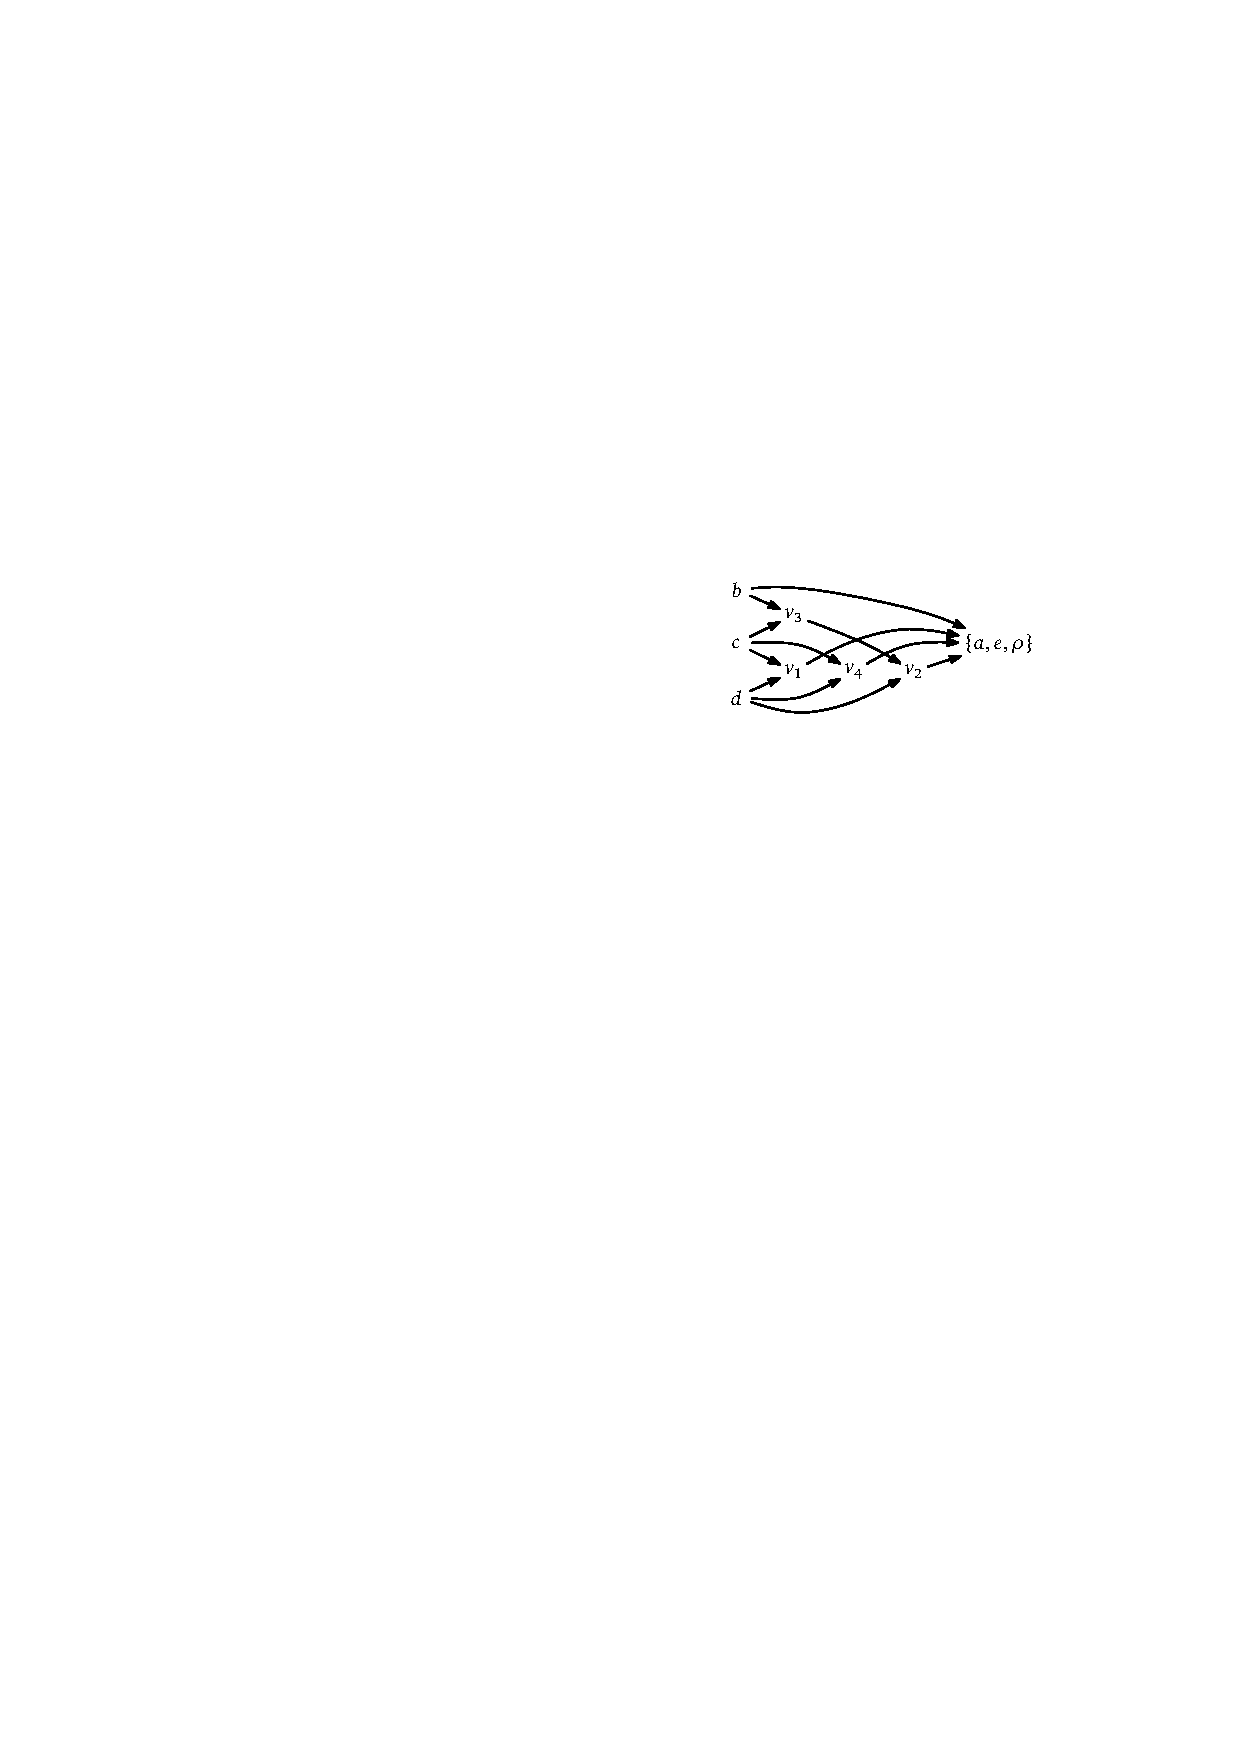
\includegraphics{../figs/ch4/signature-dag}
  \caption{The DAG $D$ used in the reconstruction of the signature $\tilde H$
    in Figure~\ref{fig:reconstruction-signature} from the description in
    Figure~\ref{fig:reconstruction-input}.}
  \label{fig:signature-dag}
\end{figure}
%-------------------------------------------------------------------------------

%-------------------------------------------------------------------------------
\begin{figure}
  \centering
  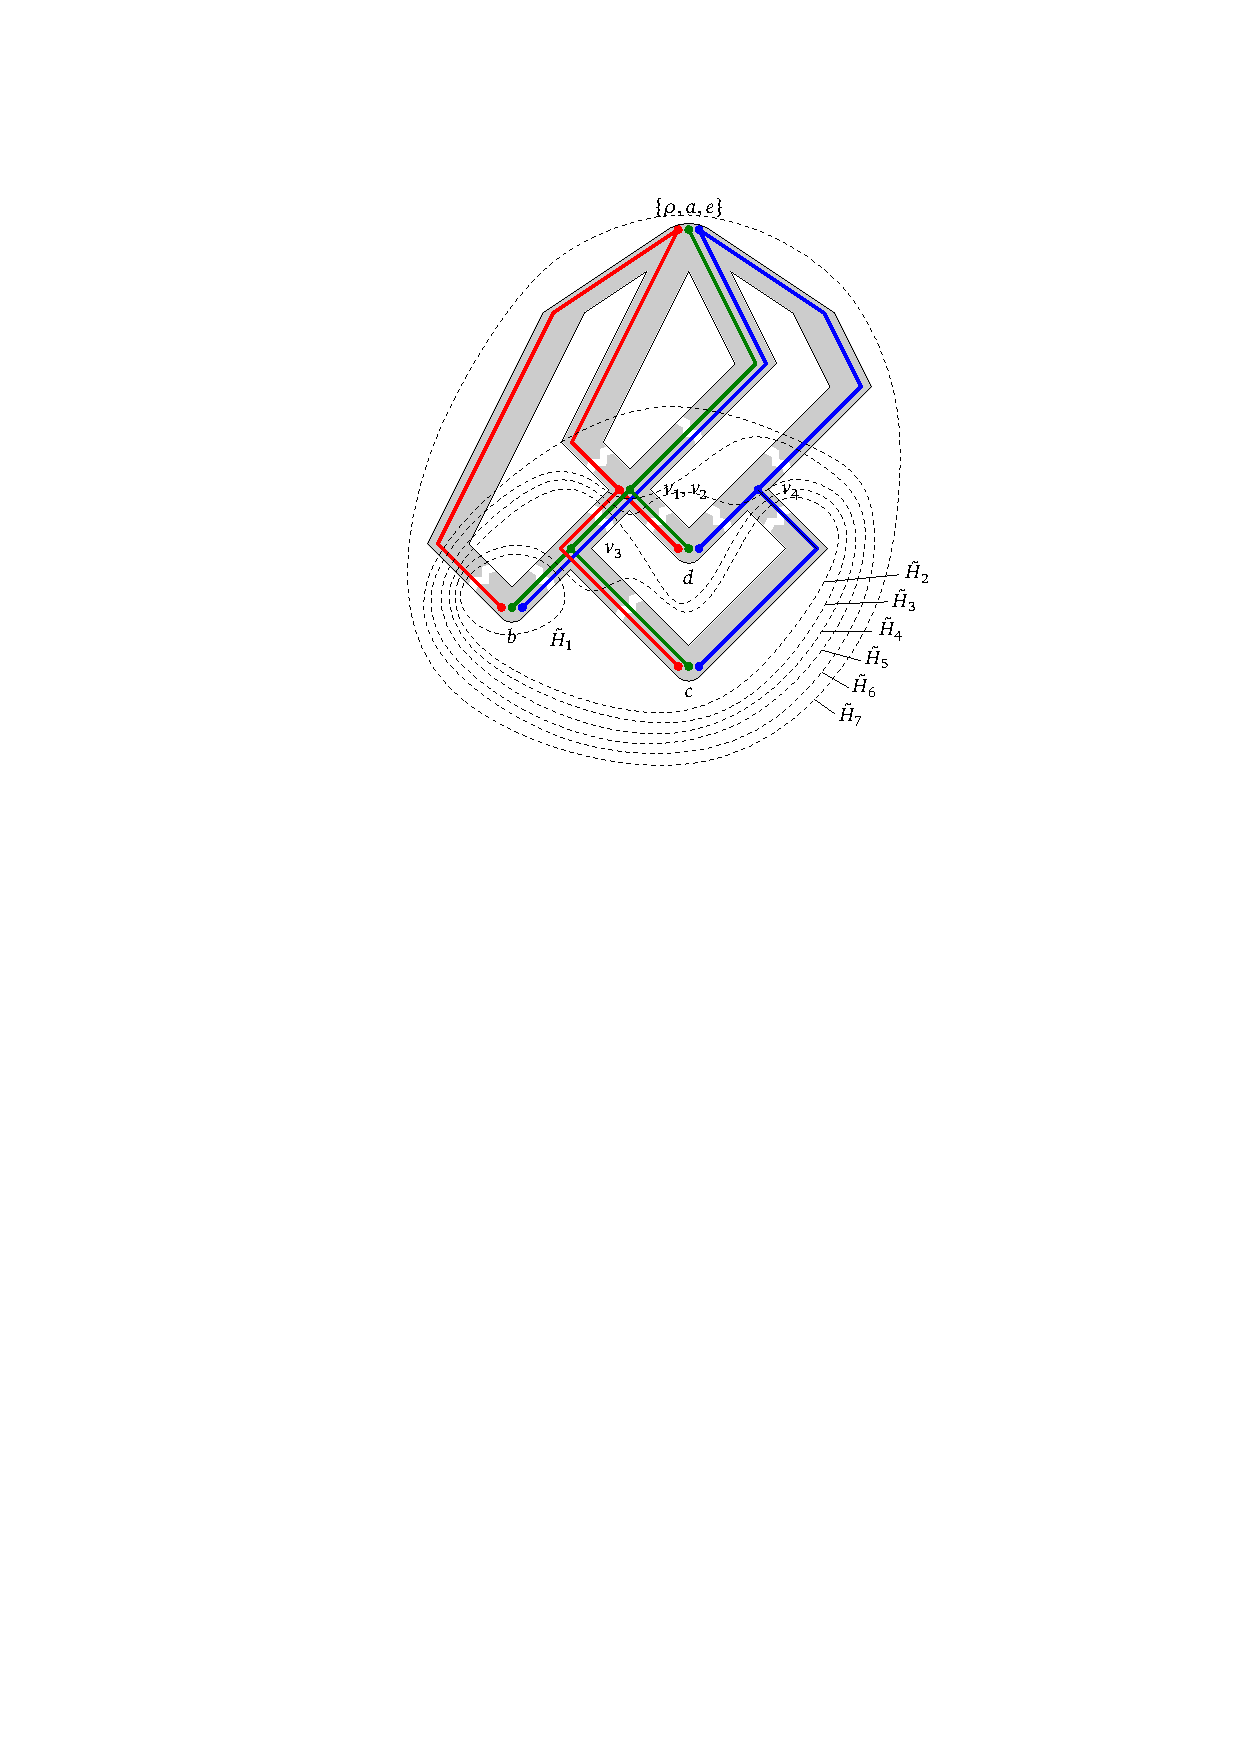
\includegraphics{../figs/ch4/reconstruction-signature}
  \caption{The signature $\tilde H$ of any CNET with the description
    $(\G, F^*, \T)$ shown in Figure~\ref{fig:reconstruction-input}.
    The {partial signatures} $\tilde H_1, \tilde H_2, \dots, \tilde H_7 = \tilde H$
    constructed incrementally are indicated by dashed lines.}
  \label{fig:reconstruction-signature}
\end{figure}
%-------------------------------------------------------------------------------

%-------------------------------------------------------------------------------
\begin{figure}
  \centering
  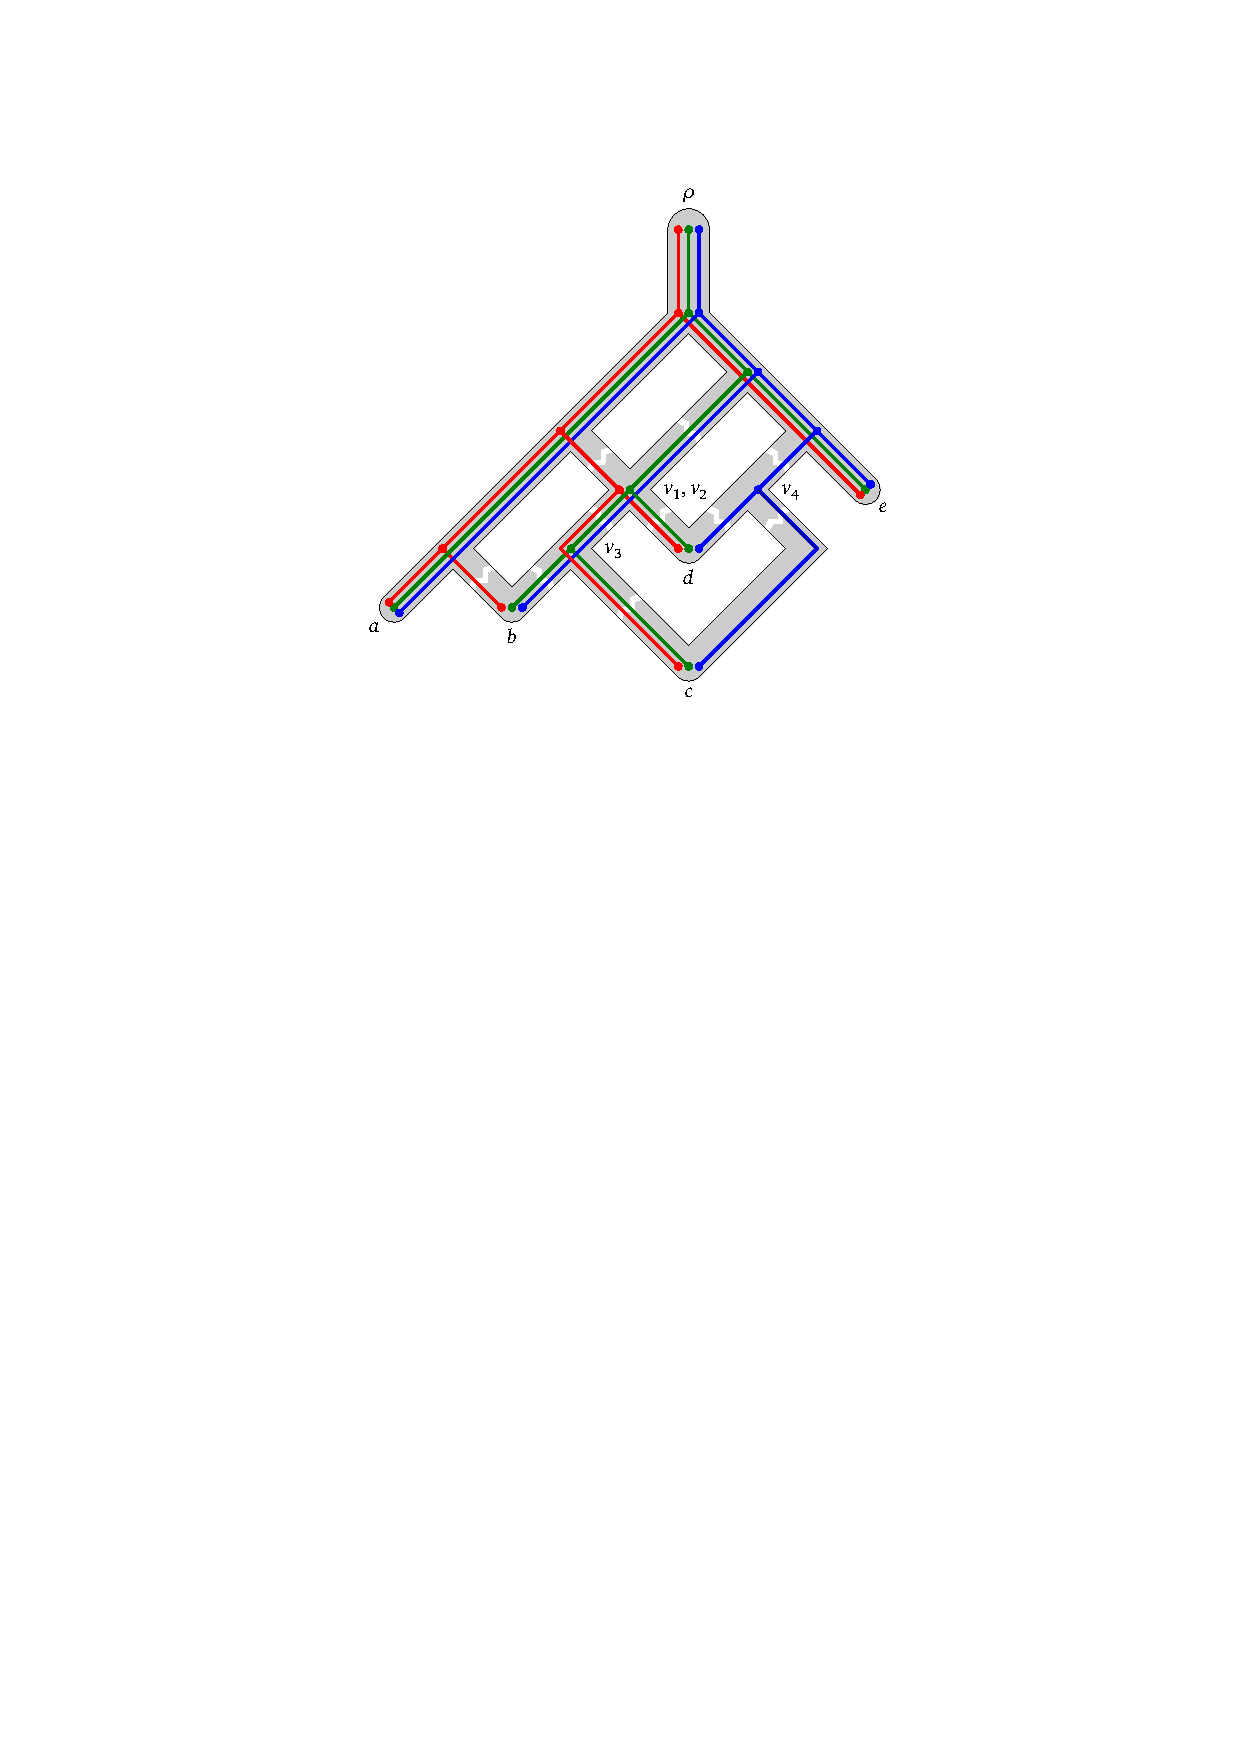
\includegraphics{../figs/ch4/reconstruction-output-network}
  \caption{The CNET obtained from the signature in
    Figure~\ref{fig:reconstruction-signature} by expanding the components
    of~$F$.}
  \label{fig:reconstruction-output}
\end{figure}
%-------------------------------------------------------------------------------

%-------------------------------------------------------------------------------
\begin{figure}
  \centering
  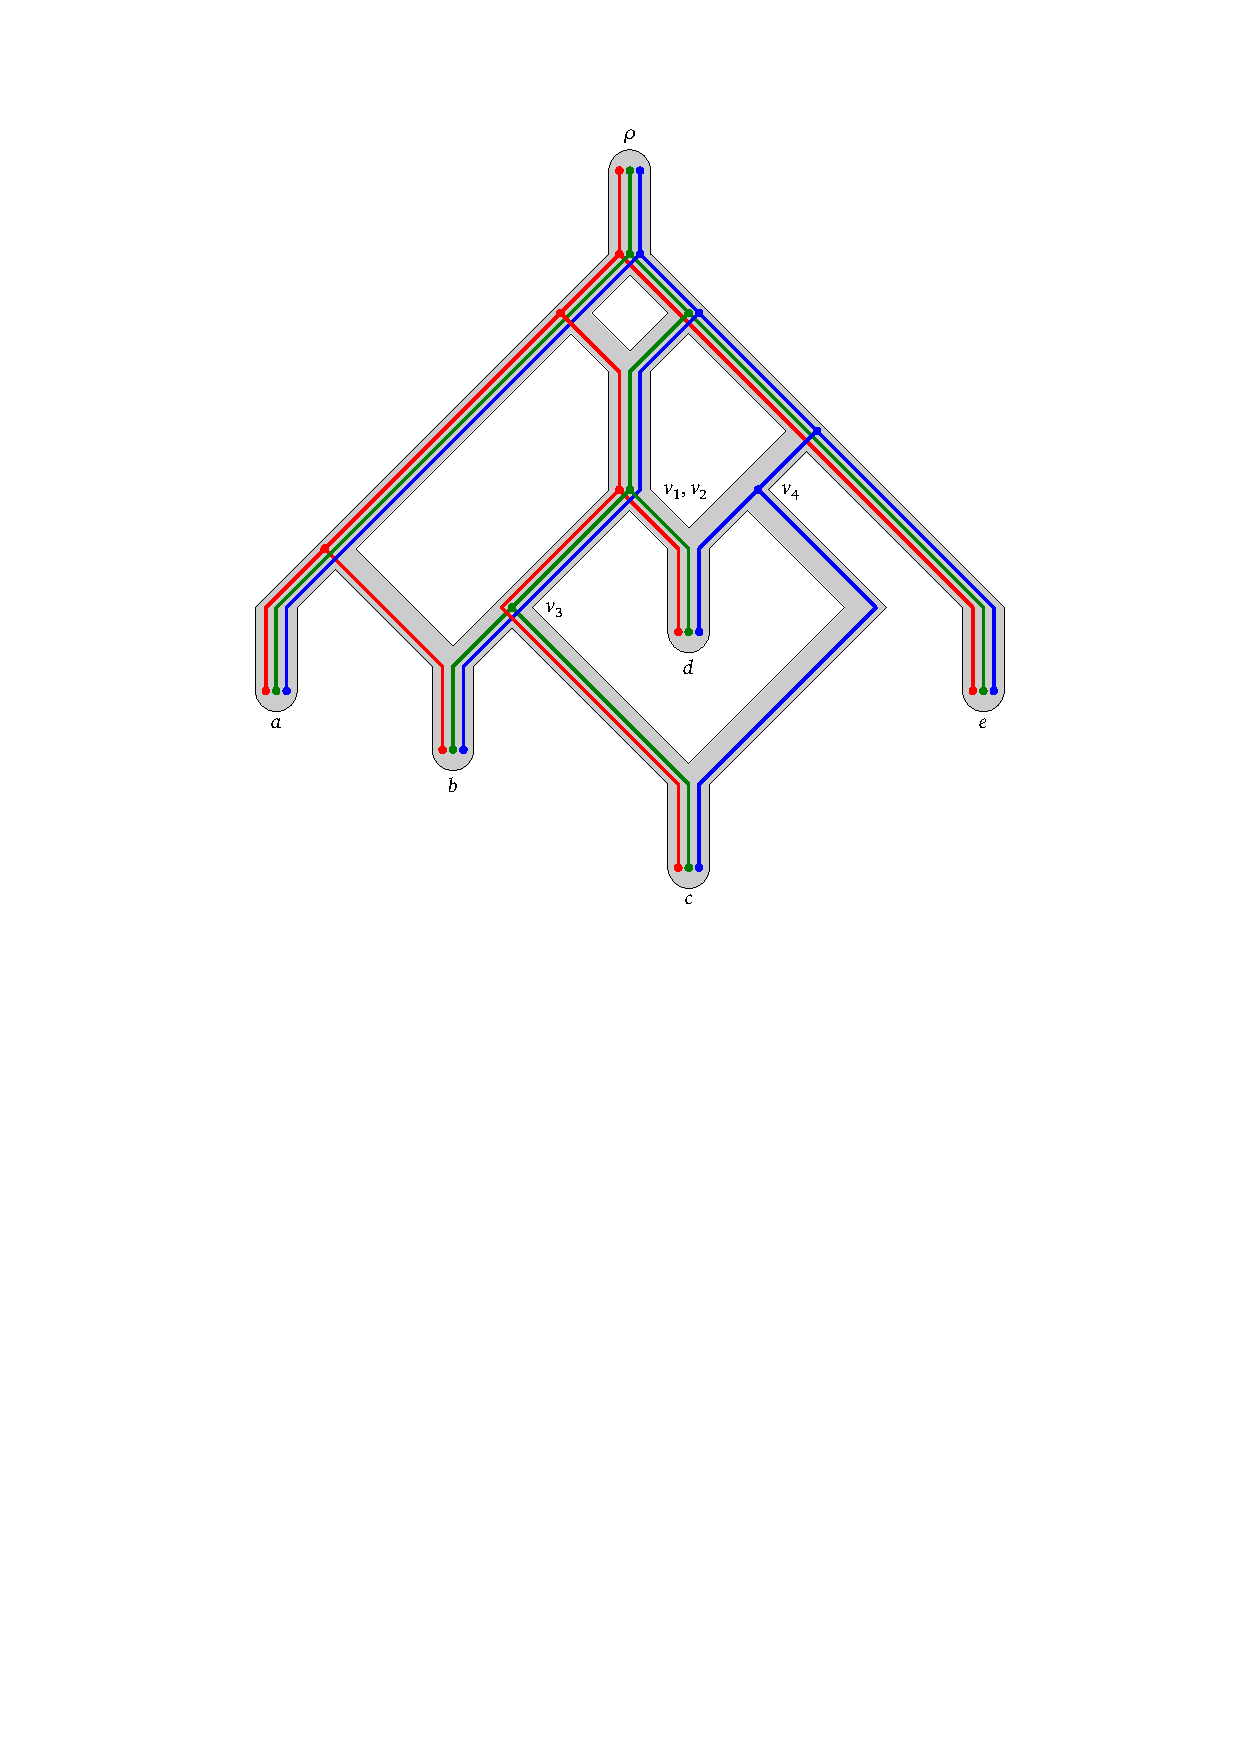
\includegraphics{../figs/ch4/reconstruction-final-network}
  \caption{The hybridization network induced by the CNET in
    Figure~\ref{fig:reconstruction-output}, obtained by separating reticulations,
    split nodes, and leaves.}
  \label{fig:reconstruction-final}
\end{figure}
%-------------------------------------------------------------------------------


Before the first iteration, we have $\bar D_0 = D$.
The only nodes with in-degree $0$ in $\bar D_0$ are $b$, $c$, and $d$.
They are all free because they have no in-edges at all.
Assume we pick $b$ as the first node to add to $\tilde H$.
We create the node $H(b)$ and add parent edges according to $b$'s wiring guess
to obtain the partial network $\tilde H_1$ in
Figure~\ref{fig:reconstruction-signature}.
Since $b$ is the root of an AAF component, it has no buddies, so
$D_1$ has the node set $\set{b}$.

$\bar D_1$ has two nodes of in-degree $0$, namely $c$ and $d$.
Both are again free.
Assume we choose $c$ as the next node to add to $D_1$ to obtain $D_2$.
Since $c$ is again the root of an AAF component, it has no buddies, so the
node set of $D_2$ is $\set{b, c}$.
We construct the graph $\tilde H_2$ in Figure~\ref{fig:reconstruction-output}
from $\tilde H_1$ by creating a node $H(c)$ and {adding} parent edges of this node
according to $c$'s wiring guess.

$\bar D_2$ has two nodes of in-degree $0$, namely $d$ and $v_3$.
Both nodes are free: $d$ is free {because it is the root of an AAF component}; $v_3$ is free because $\tilde H_2$ has two root
edges above $H(b)$ and $H(c)$, which are children of $v_3$ in the green tree,
and the top endpoints of both edges are coloured green by the wiring guesses
for $b$ and $c$.
Let us assume we choose $v_3$ as the next node to add to $D_2$ to obtain
$D_3$.
We create the node $H(v_3)$ by identifying the top endpoints of the two green
parent edges of $H(b)$ and $H(c)$ and add a parent edge above $H(v_3)$
according to $v_3$'s wiring guess.
This gives the graph $\tilde H_3$ shown in
Figure~\ref{fig:reconstruction-signature}.
Since the only tree common to the colour sets of the parent edges of $H(b)$
and $H(c)$ is the green one, $v_3$ has no buddies.
Thus, $D_3$ has node set $\set{b, c, v_3}$.

$\bar D_3$ has $d$ as its only in-degree-$0$ node, and $d$ is free.
We obtain $D_4$ by adding $d$ to $D_3$.
Node $d$ has no buddies because it is the root of an AAF component.
To obtain $\tilde H_4$ from $\tilde H_3$, we create the node
$H(d)$ and add parent edges according to $d$'s wiring guess.

$\bar D_4$ has three nodes of in-degree $0$, namely $v_1$, $v_2$, and $v_4$.
The two child edges of $v_1$ are represented by red parent edges of
$H(v_3)$ and $H(d)$ in $\tilde H_4$.
According to the wiring guesses for $v_3$ and $d$, their top endpoints are
red.
Since $v_1$ belongs to the red tree, $v_1$ is free.
The same two edges also represent the child edges of $v_2$.
However, $v_2$ is green and, thus, is not free.
Finally, the two child edges of $v_4$ are represented by the blue parent
edges of $H(c)$ and $H(d)$, both of which have blue top endpoints according
to the wiring guesses for $c$ and $d$.
Thus, $v_4$ is also free.
Assume we choose $v_4$ as the next node to add to $D_4$ to obtain $D_5$.
We create the node $H(v_4)$ in $\tilde H_5$ by identifying the top endpoints
of the blue parent edges of $H(c)$ and $H(d)$ and then create a parent edge
of $H(v_4)$ according to $v_4$'s wiring guess.
This produces the graph $\tilde H_5$ in
Figure~\ref{fig:reconstruction-signature}.
Since the colour sets of the two child edges of $H(v_4)$ have only the blue tree
in common, $v_4$ has no buddies and $D_5$ has node set
$\set{b, c, d, v_3, v_4}$.

Nodes $v_1$ and $v_2$ are the only nodes of in-degree $0$ in $\bar D_5$. Just as in $\bar D_4$, $v_1$ is free and $v_2$ is not. Thus, we choose $v_1$ as the node to add  to $D_5$ to obtain $D_6$. The two child edges of $v_1$ are represented by the red parent edges of $H(v_3)$ and $H(d)$ in $\tilde H_5$. We identify their top endpoints to create the node $H(v_1)$ and add parent edges according to the wiring guess for $v_1$. This produces the graph $\tilde H_6$ in Figure~\ref{fig:reconstruction-signature}. Now observe that the two child edges of $H(v_1)$ in $\tilde H_6$ are also coloured green. Thus, we identify the node that is the parent of the two edges of the green tree represented by these child edges, which is node $v_2$. Node $v_2$ becomes a buddy of $v_1$ and is added to $D_5$ along with $v_1$ to obtain $D_6$. Thus, $D_6$ has node set $\set{b, c, d, v_1, v_2, v_3, v_4}$. Note that making $v_1$ and $v_2$ buddies does not create any conflicts because they both have the same wiring guess in $\G$. 

Finally, the only node remaining in $\bar D_6$ is $\set{a, e, \rho}$. The root edges of $\tilde H_6$ represent exactly the set of pendant edges of the AAF component $\set{a, e, \rho}$ in the three input trees, so $\set{a, e, \rho}$ is free in $\bar D_6$. We create a node $H(\set{a, e, \rho})$ in $\tilde H_7$ by identifying the top endpoints of all root edges of $\tilde H_6$. Since there is no wiring guess for $\set{a, e, \rho}$ in $\G$, we do not add any parent edges to $H(\set{a, e, \rho})$, and $\tilde H_7 = \tilde H$ is the final signature.

It is easily verified that we would have obtained the exact same signature had we chosen different nodes to add to $D_i$ in iterations where $\bar D_i$ contained more than one free node.

%-------------------------------------------------------------------------------
\paragraph{Lemma~\ref{lem:network-from-description}: Expanding AAF components.}
%-------------------------------------------------------------------------------

In our example, the only non-trivial AAF component to be expanded is the component $\set{a, e, \rho}$. This component has two non-root edges. Let $f_a$ be the parent edge of $a$, and let $f_e$ be the parent edge of $e$ in this component. In $\tilde H$, the node $H(\set{a, e, \rho})$ has four child edges: a red parent edge $e_1$ of $H(b)$, a red parent edge $e_2$ of $H(v_1) = H(v_2)$, a green-blue parent edge $e_3$ of $H(v_1) = H(v_2)$, and a blue parent edge $e_4$ of $H(v_4)$. Edges $e_1$ and $e_2$ attach to $f_a$ in the red tree and do not represent any edges in any other trees, so we add them to $E_{f_a}$. Edge $e_3$ attaches to $f_e$ in the green and the blue tree, so there is no conflict and we add it to $E_{f_e}$. Edge $e_4$ attaches to $f_e$ in the blue tree and does not represent any {edge} in any other {tree}, so we add it to $E_{f_e}$. 

The DAG $D_{f_a}$ has two nodes representing edges $e_1$ and $e_2$ with an edge from $e_2$ to $e_1$ because $e_2$ attaches to $f_a$ above $e_1$ in the red tree. A topological ordering of $D_{f_a}$ places these edges in the order $\seq{e_2, e_1}$, and {this} is the order in which we attach $e_2$ and $e_1$ to $f_a$.

The DAG $D_{f_e}$ has two nodes representing edges $e_3$ and $e_4$ with an edge from $e_3$ to $e_4$ because $e_3$ attaches to $f_e$ above $e_4$ in the blue tree. The green tree does not impose any conflicting ordering constraints because only edge $e_3$ belongs to this tree. A topological ordering of $D_{f_e}$ places $e_3$ and $e_4$ in the order $\seq{e_3, e_4}$, and this is the order in which we attach $e_3$ and $e_4$ to $f_e$. The result is the CNET shown in Figure~\ref{fig:reconstruction-output}. 
{Finally, the hybridization network induced by this CNET is shown in Figure~\ref{fig:reconstruction-final}.}



%-------------------------------------------------------------------------------
%\section{Conclusion}\label{sec:concl}
%-------------------------------------------------------------------------------

It seemed natural enough to try to reconstruct a hybridization network from the corresponding AAF and {to guess} the wiring structure that determines how the AAF components need to be glued together to achieve this. In the case of two trees, no guessing is required: the AAF carries the necessary information. For more than two trees, there are only a constant number of choices for the wiring of the root of each component, so with $\Oh(k)$ components, one obtains an $\Oh(c^k \cdot \poly(n))$ time algorithm. Unfortunately, guessing the wiring structure of AAF components turned out not to be enough, even for three trees, because there are examples of three input trees such that every optimal network displaying these trees contains an \emph{invisible component}: a group of nodes that are isolated from all taxa once all hybridization edges are deleted, see Figure~\ref{fig:invisible} {in the introduction}. We call these components invisible because they are not represented in any form in the AAF.

Guessing the number and structure of these invisible components seems extremely challenging. In this chapter, we showed that one can get away without having to guess these components in the case of three trees because, for three trees, these components are not invisible after all: They may not be represented in the AAF, but they are present as nodes in the three input trees, at least as long as we consider only canonical networks (and we have shown that we may do this without loss of generality). This is the key to our $\Oh(c^k \cdot \poly(n))$-time algorithm for three trees. Unfortunately, it appears that we simply scraped by.\comment{LI}{Scraped by???} While the framework of our algorithm extends to more than three trees, it seems that already for four trees, there are input instances where the optimal network includes truly invisible nodes: nodes whose only purpose is to change the way in which edges of the tree images are braided together along network edges, see Figure~\ref{fig:braided}. Thus, the main open problem is to discover structural properties that, while unlikely to eliminate the need to guess the existence of these braiding structures in the network altogether, at least limit the number of possible guesses to be explored.

  %-----------------------------------------------------------------------------
  \begin{figure}[h]
    \centering
    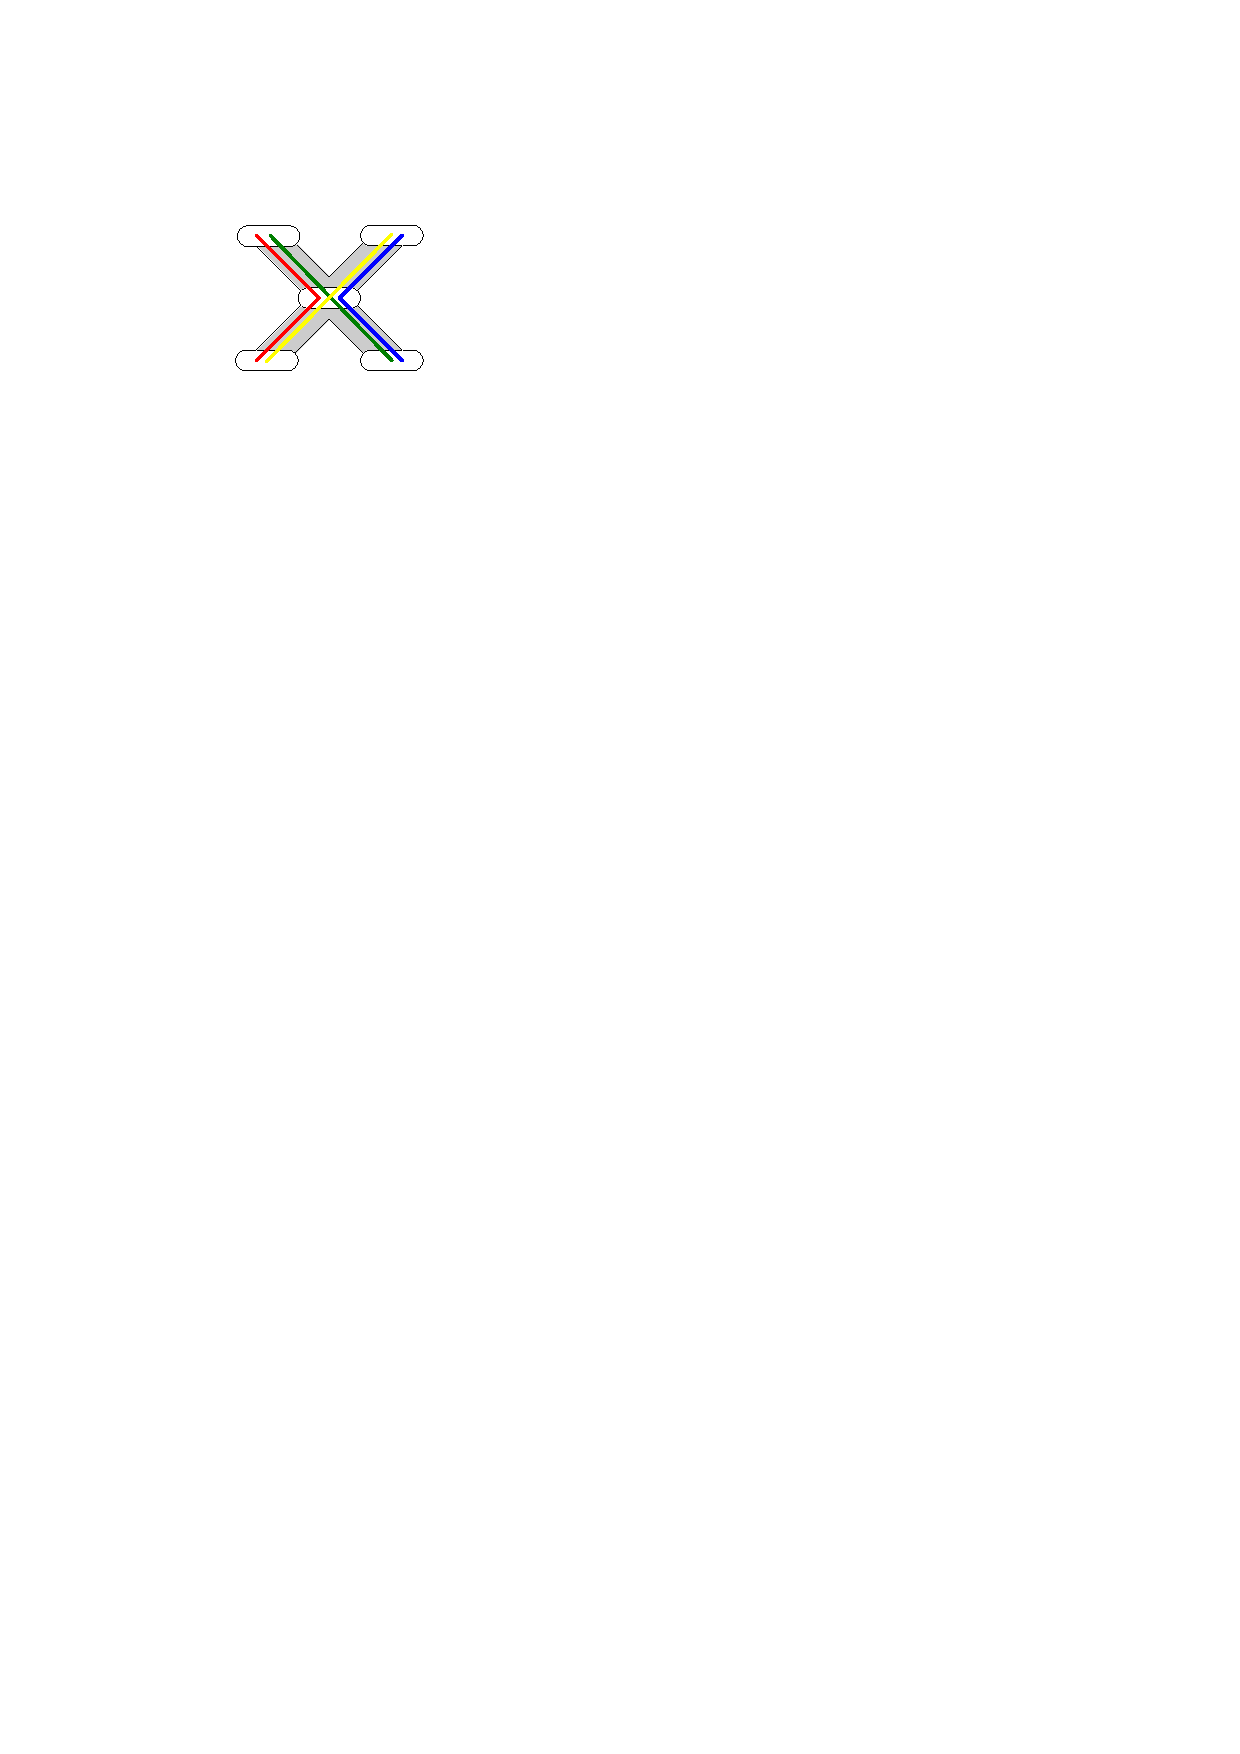
\includegraphics{../figs/ch4/braided}
    \caption{A ``truly invisible'' node of a network with four trees embedded in it. None of the four trees branches in this network node.}
    \label{fig:braided}
  \end{figure}
  %-----------------------------------------------------------------------------


Another interesting question that arises from our work is whether guessing the wiring of the extended AAF components as part of the reconstruction is necessary at all, at least in the case of three trees. Since all these components are visible in the input trees, it could be possible that one can construct the entire network directly from the AAF, that is, as in the case of two trees, the hard core of the problem is finding the right AAF. However, we conjecture that this is not the case: i.e., that even given the deletion AAF of an optimal hybridization network for the three input trees, it remains NP-hard to find the network. 